\documentclass{article}
\usepackage[utf8]{inputenc}
\usepackage[table,xcdraw]{xcolor}
\usepackage{fancyhdr}
\usepackage{geometry} % para controlar márgenes
\usepackage[spanish]{babel}
\usepackage{listings}
\usepackage{xcolor}
\usepackage{url}
\usepackage{graphicx}
\usepackage{float}
\usepackage{longtable}
\usepackage{colortbl}
\usepackage{multirow}
\usepackage[table]{xcolor}
\usepackage{tabularx}
\usepackage{colortbl}


%%%%%%%%%%%%%%%%%%%%%%%%%%%%%%%%%%%%%%%%%%%%%%%%%%%%%%%%%%%%%%%%%%%%%%%%%%%%%%%%%%%%%
%%%%%%%%%%%%%%%%%%%%%%%%%%%%%%%%%%%%%%%%%%%%%%%%%%%%%%%%%%%%%%%%%%%%%%%%%%%%%%%%%%%%%

\definecolor{tablebackground}{rgb}{0.8, 0, 0}
\definecolor{tabledictionariesbackground}{RGB}{122, 161, 194}
\definecolor{codebackground}{rgb}{0.95, 0.95, 0.92}


\newcommand{\itemStudent}{\begin{tabular}{l}
Bedregal Coaguila, Karla M. \\
Llaique Chullunquia, Jack F. \\
Ramos Ochochoque, Elkin E. \\
Vilca Huarca, Laura L. \\
\end{tabular}}
\newcommand{\itemTittle}{”Sistema de Inscripciones para la Cuna Jardín UNSA”}
\newcommand{\itemCourse}{Programación Web 2}
\newcommand{\itemCourseCode}{1702122}
\newcommand{\itemSemester}{III}
\newcommand{\itemUniversity}{Universidad Nacional de San Agustín de Arequipa}
\newcommand{\itemFaculty}{Facultad de Ingeniería de Producción y Servicios}
\newcommand{\itemDepartment}{Departamento Académico de Ingeniería de Sistemas e Informática}
\newcommand{\itemSchool}{Escuela Profesional de Ingeniería de Sistemas}
\newcommand{\itemAcademic}{2025 - A}
\newcommand{\itemInput}{22 Julio 2025}
\newcommand{\itemOutput}{27 Julio 2025}
%%%%%%%%%%%%%%%%%%%%%%%%%%%%%%%%%%%%%%%%%%%%%%%%%%%%%%%%%%%%%%%%%%%%%%%%%%%%%%%%%%%%%
%%%%%%%%%%%%%%%%%%%%%%%%%%%%%%%%%%%%%%%%%%%%%%%%%%%%%%%%%%%%%%%%%%%%%%%%%%%%%%%%%%%%%


% Márgenes más ajustados si deseas, pero no obligatorio
\geometry{top=2.5cm, bottom=2.5cm, left=2.5cm, right=2.5cm}

%Definimos estilo para codigo tree
\lstdefinestyle{ascii-tree}{
    basicstyle=\ttfamily\footnotesize,
    literate={├}{|}1 {─}{-}1 {└}{+}1,
    numbers=none
}

%Definimos estilo para las lineas de codigo
\lstdefinestyle{mystyle}{
    numbers=left,
    numberstyle=\tiny\color{gray},
    stepnumber=1,
    numbersep=10pt,
    backgroundcolor=\color{gray!10},
    showspaces=false,
    showstringspaces=false,
    showtabs=false,
    frame=tb,
	aboveskip=2mm,
	belowskip=2mm,
    tabsize=1,
    captionpos=b,
    breaklines=true,
    breakatwhitespace=false,
    keywordstyle=\color{purple},
    commentstyle=\color{gray}\itshape,
    stringstyle=\color{blue},
    basicstyle=\ttfamily\footnotesize,
} 

\lstset{style=mystyle}
\lstdefinestyle{ascii-tree}{
    literate={├}{|}1 {─}{--}1 {└}{+}1,
    numbers=none,
  }
% CONFIGURACIÓN ENCABEZADO
\pagestyle{fancy}

% Líneas normales (0.4pt) tamaño predeterminado
\renewcommand{\headrulewidth}{0.4pt}
\renewcommand{\footrulewidth}{0.4pt}

% Altura suficiente para el encabezado y pie
\setlength{\headheight}{46pt}
\setlength{\footskip}{20pt}

% Encabezado de pagina
\fancyhead[L]{\raisebox{0.3\height}{
\includegraphics[width=2.7cm]{images/sistemas-logo.png}}}
\fancyhead[C]{\fontsize{7}{7}\selectfont	\itemUniversity \\ \itemFaculty \\ \itemDepartment \\ \itemSchool \\ \textbf{\itemCourse}}
\fancyhead[R]{\raisebox{0.1\height}{
\includegraphics[width=1.2cm]{images/abet-logo.png}}}

% Pie de página
\fancyfoot[L]{ Proyecto Final "SICU"}
\fancyfoot[C]{ Pág. \thepage}
\fancyfoot[R]{ Programación Web 2}

\begin{document}

    %Catatula del trabajo
    \begin{center}
    {\LARGE \textbf{\\Proyecto Final}}\\
    \vspace{0.5em}
    {\large \textbf{SICU:} \textbf{\itemTittle}}
    \vspace{1.5em}

     % Tabla de nota
    \noindent
    \makebox[16.48cm][r]{%
        \begin{tabular}{|>{\centering\arraybackslash}m{2.5cm}|}
            \hline 
            \rowcolor{tablebackground}
            \color{white} \textbf{Nota}  \\
            \hline 
            \\[30pt]
            \hline 			
        \end{tabular}
    }
    \vspace{1.5em}
    
    % Tabla de docente, escuela y asignatura
    \begin{tabular}{|>{\centering\arraybackslash}m{5cm}|>{\centering\arraybackslash}m{5cm}|>{\centering\arraybackslash}m{5cm}|}
        \hline
        \rowcolor{tablebackground}
        \textbf{\color{white}Estudiantes} & \textbf{\color{white}Escuela} & \textbf{\color{white}Asignatura} \\
        \hline
        \itemStudent &
        \shortstack{\\\\\\\\\\Escuela Profesional de Ingeniera \\de Sistemas} &
        \shortstack{\\\\\\\\\itemCourse\\Semestre: \itemSemester\\Código: \itemCourseCode} \\
        \hline
    \end{tabular}
    \vspace{1.5em}

    % Tabla de fechas
    \begin{tabular}{|>{\centering\arraybackslash}m{5cm}|>{\centering\arraybackslash}m{5cm}|>{\centering\arraybackslash}m{5cm}|}
        \hline
        \rowcolor{tablebackground}
        \textbf{\color{white}Semestre académico} & \textbf{\color{white}Fecha de inicio} & \textbf{\color{white}Fecha de entrega} \\
        \hline
           \itemAcademic  & \itemInput & \itemOutput \\
        \hline
    \end{tabular}
    \vspace{1.5em}

\end{center}
\tableofcontents
    \newpage


%%%%%%%%%%%%%%%%%%%%%%%%%%%%% CUERPO DEL INFORME %%%%%%%%%%%%%%%%%%%%%%%%%%%%%
\section{Introducción}
    \subsection{Tipo de Sistema}
        El presente proyecto, titulado \textbf{SICU - Sistema de Inscripciones para la Cuna Jardín UNSA}, consiste en una aplicación web desarrollada con una arquitectura de cliente-servidor. El backend ha sido implementado utilizando el framework \textbf{Django}, haciendo uso del módulo \textbf{Django REST Framework (DRF)} para la creación de APIs, mientras que el frontend ha sido construido con el framework \textbf{Vue}, lo que permite una experiencia de usuario dinámica y moderna.
        El sistema está dirigido al personal administrativo de la \textbf{Cuna Jardín UNSA}, con el propósito de digitalizar y automatizar el proceso de inscripción de niños entre 0 y 5 años. Mediante esta plataforma se busca reemplazar los procedimientos manuales tradicionales, reduciendo errores, mejorando la organización institucional y optimizando el tiempo dedicado al registro y seguimiento de estudiantes, apoderados, docentes y cursos.
        La solución planteada facilita el acceso remoto a la información, gracias a su despliegue como aplicación web, y sienta las bases para futuras extensiones del sistema, como la integración con otros servicios, la generación de reportes o la incorporación de módulos gráficos.
    \subsection{Justificación}
        La implementación de un sistema web para la gestión de inscripciones en la Cuna Jardín UNSA responde a la necesidad de modernizar procesos administrativos que, hasta el momento, se realizaban de forma manual. Este cambio representa múltiples beneficios, entre los cuales destacan:
        \begin{itemize}
            \item \textbf{Reducción de errores:} Al eliminar el registro manual, se disminuyen los errores en la carga y gestión de datos, mejorando el seguimiento individual de cada niño inscrito.
            \item \textbf{Ahorro de tiempo:} La automatización de procesos permite realizar inscripciones, consultas y actualizaciones de manera ágil y eficiente.
            \item \textbf{Mejor organización:} El sistema facilita la generación de reportes estadísticos y el control ordenado de la información, apoyando la toma de decisiones administrativas.
            \item \textbf{Accesibilidad:} Al tratarse de una aplicación web, los responsables del sistema pueden acceder a la plataforma desde cualquier lugar con conexión a Internet.
            \item \textbf{Escalabilidad:} Gracias a su arquitectura modular, el sistema permite futuras mejoras e integraciones sin comprometer su funcionamiento actual.
        \end{itemize}
    \subsection{Objetivo General}
        \begin{itemize}
            \item Desarrollar un sistema informático que permita la administración digital de inscripciones en la Cuna
            Jardín UNSA, con una estructura orientada a objetos para facilitar su mantenimiento y escalabilidad.
        \end{itemize}
    \subsection{Objetivos Específicos}
        \begin{itemize}
            \item Modelar entidades clave del dominio educativo: estudiantes, apoderados, docentes, cursos e inscripciones.
            \item Implementar operaciones para registrar, modificar, consultar y eliminar información relevante.
            \item Asegurar integridad y consistencia de datos mediante reglas definidas en las clases.
            \item Preparar el sistema para su futura integración con interfaces gráficas o web.
        \end{itemize}

\section{Arquitectura del Sistema}
    \subsection{Tecnologías Utilizadas}
        \begin{itemize}
            \item \textbf{Git y GitHub:} Control de versiones y repositorios remotos.
            \item \textbf{Python 3.13:} Lenguaje principal para el backend.
            \item \textbf{Django 5:} Framework web backend en Python.
            \item \textbf{Django REST Framework (DRF):} Creación de APIs RESTful.
            \item \textbf{Vue 3:} Framework frontend basado en JavaScript.
            \item \textbf{JavaScript:} Lenguaje tipado para el desarrollo en Vue.
            \item \textbf{Bootstrap 5:} Estilos e interfaces responsivas.
            \item \textbf{Visual Studio Code:} Editor de código fuente.
            \item \textbf{PostgreSQL:} Base de datos relacional para el backend.
            \item \textbf{Supabase:} Base de datos PostgreSQL en la nube.
            \item \textbf{SoapUI:} Pruebas de servicios REST.
            \item \textbf{Vercel (plan gratuito):} Despliegue del backend en la nube.
            \item \textbf{Netlify (plan gratuito):} Despliegue del frontend en la nube.
            \item \textbf{Navegadores Web:} Chrome, Firefox, Edge, Brave, Opera.
            \item \textbf{Sistemas operativos:} Windows 11 y Linux.
        \end{itemize}
    \subsection{Estructura del Proyecto Backend}
    \begin{itemize}	
		\item El contenido que se entrega para la parte de Backend en este laboratorio es el siguiente:
	\end{itemize}
        \begin{lstlisting}[style=ascii-tree, numbers=none]
    Backend/
    |-- AppCuna
    |   |-- admin.py
    |   |-- apps.py
    |   |-- migrations
    |   |   |-- Student.py
    |   |   |-- Inscription.py
    |   |   |-- ...
    |   |-- models
    |   |-- serializers.py
    |   |-- urls.py
    |   \-- views.py
    |-- manage.py
    |-- MyDjangoProject
    |   |-- settings.py
    |   \-- urls.py
    |-- venvf
    |   |-- bin
    |   |-- include
    |   |-- lib
    |   |-- pyvenv.cfg
    |-- requirements.txt
        \end{lstlisting}


    \subsection{Estructura del Proyecto Frontend}
        \begin{itemize}	
            \item El contenido que se entrega para la parte de Frontend en este laboratorio es el siguiente:
        \end{itemize}
            \begin{lstlisting}[style=ascii-tree, numbers=none]
    Frontend/
    |-- public
    |   |-- index.html
    |   |-- favicon.ico
    |   \-- _redirects
    |-- src
    |   |-- App.vue
    |   |-- main.js
    |   |-- assets
    |   |   \-- logo.png
    |   |-- components
    |   |   |-- HelloWorld.vue
    |   |   \-- common/
    |   |-- router
    |   |   \-- index.js
    |   |-- services
    |   |   \-- api.js
    |   |-- store
    |   |   \-- index.js
    |   \-- views
    |       |-- Dashboard.vue
    |       |-- Login.vue
    |       |-- Profile.vue
    |       |-- Students.vue
    |       |-- Grades.vue
    |       |-- Attendance.vue
    |       |-- Announcement.vue
    |       |-- Payments.vue
    |       |-- Inscriptions.vue
    |       |-- Teachers.vue
    |       |-- Courses.vue
    |       |-- Documents.vue
    |       |-- Periods.vue
    |       |-- Chats.vue
    |       |-- Home.vue
    |       |-- about-us.vue
    |       |-- Workloads.vue
    |       \-- user/
    |-- package.json
    |-- package-lock.json
    |-- vue.config.js
    |-- netlify.toml
    \-- README.md
            \end{lstlisting}
    \subsection{Separación Cliente - Servidor (Vue + Django)}
        El sistema fue desarrollado bajo una arquitectura de cliente-servidor, dividiendo claramente las responsabilidades entre el frontend (cliente) y el backend (servidor).
        \begin{itemize}
            \item El \textbf{backend}, implementado con \textbf{Django 5} y \textbf{Django REST Framework}, se encarga de la lógica del negocio, la gestión de la base de datos, las reglas de validación y la exposición de los datos mediante una \textbf{API RESTful}. Esta API ofrece múltiples endpoints que permiten consultar, registrar, modificar y eliminar información relacionada con estudiantes, apoderados, docentes, cursos, inscripciones, entre otros.
            \item El \textbf{frontend}, desarrollado con \textbf{Vue 3}, consume estos servicios a través de peticiones HTTP (principalmente métodos GET y POST). Vue se encarga de renderizar las vistas del sistema, gestionar la navegación del usuario, validar formularios en el cliente y mostrar respuestas o mensajes.
        \end{itemize}
        Esta separación permite una mayor flexibilidad, ya que ambas partes pueden desarrollarse, probarse y desplegarse de manera independiente. Además, mejora la escalabilidad del sistema, facilitando la integración futura con otros clientes, como aplicaciones móviles u otros sistemas web.

\section{Modelado de Datos}
    \subsection{Entidades y relaciones}
        \subsubsection{Student}
        Este modelo representa a los estudiantes (niños) inscritos en la Cuna Jardín. Incluye información personal, de salud, y vínculos parentales. Contiene validaciones internas para asegurar la integridad en campos como limitaciones físicas o seguro médico.

        \subsubsection{Mother}
        Modelo que almacena la información detallada de las madres. Incluye datos personales, laborales, nivel de instrucción y vínculo con la universidad. Al registrar a una madre se puede crear automáticamente un usuario asociado y enviarle sus credenciales por correo.

        \subsubsection{Father}
        (Nota: aunque no se muestra su definición, se infiere su existencia). Representa al padre del estudiante y se relaciona desde el modelo `Student`.

        \subsubsection{Teacher}
        Representa a los docentes que dictan cursos en la Cuna. Al igual que las madres, se puede generar un usuario automáticamente y enviar credenciales. Se almacena su experiencia, formación y vínculo con la universidad.

        \subsubsection{Course}
        Contiene información sobre los cursos disponibles, como nombre, código, créditos, semestre y año. Es un modelo fundamental para la asignación de cargas docentes.

        \subsubsection{Period}
        Define los periodos académicos, como “2025-I”. Se puede activar un periodo para señalar cuál está vigente en el sistema.

        \subsubsection{Workload}
        Asocia a un docente con un curso y un periodo académico, incluyendo modalidad, sección, capacidad y horario. Es clave para organizar las inscripciones de los estudiantes.

        \subsubsection{Inscription}
        Representa la inscripción de un estudiante a una carga académica (workload). Incluye controles de unicidad para evitar inscripciones duplicadas y permite validaciones personalizadas.

        \subsubsection{Grade}
        Permite registrar notas de evaluaciones de los estudiantes en distintos tipos: exámenes, prácticas, tareas, etc. Soporta validaciones, ponderaciones y cálculo porcentual.

        \subsubsection{Attendance}
        Almacena la asistencia diaria del estudiante en una determinada inscripción. Registra si estuvo presente, ausente o llegó tarde. Asegura que no se duplique la asistencia por fecha.

        \subsubsection{Announcement}
        Gestiona los anuncios enviados por los docentes a los estudiantes en una carga académica. Cada anuncio tiene un título, contenido y fecha de publicación.

        \subsubsection{Chat}
        Modelo que permite la comunicación entre usuarios. Almacena el remitente, destinatario, mensaje y momento del envío. Está vinculado a una carga académica.

        \subsubsection{Document}
        Permite que los docentes adjunten archivos relevantes a un curso. Guarda el título, descripción, archivo y fecha de subida.

        \subsubsection{Payment}
        Registra los pagos realizados por los estudiantes. Almacena concepto, monto, fecha, estado del pago, número de recibo y comprobante digitalizado.

        \vspace{0.5cm}
        \textbf{Resumen de Relaciones:}\\
        Los modelos se relacionan entre sí principalmente por claves foráneas. `Student` se relaciona con `Mother` y `Father`. Los docentes (`Teacher`) se asocian con cursos y periodos a través de `Workload`. Los estudiantes se inscriben a cargas académicas mediante `Inscription`, y en base a estas se generan registros de notas (`Grade`), asistencias (`Attendance`), y pagos (`Payment`). El sistema también admite anuncios, documentos y mensajería interna para enriquecer la experiencia educativa.

    \subsection{Diagrama Entidad-Relación}
        \subsubsection{Estructura Académica}
            \begin{figure}[H]
                \centering
                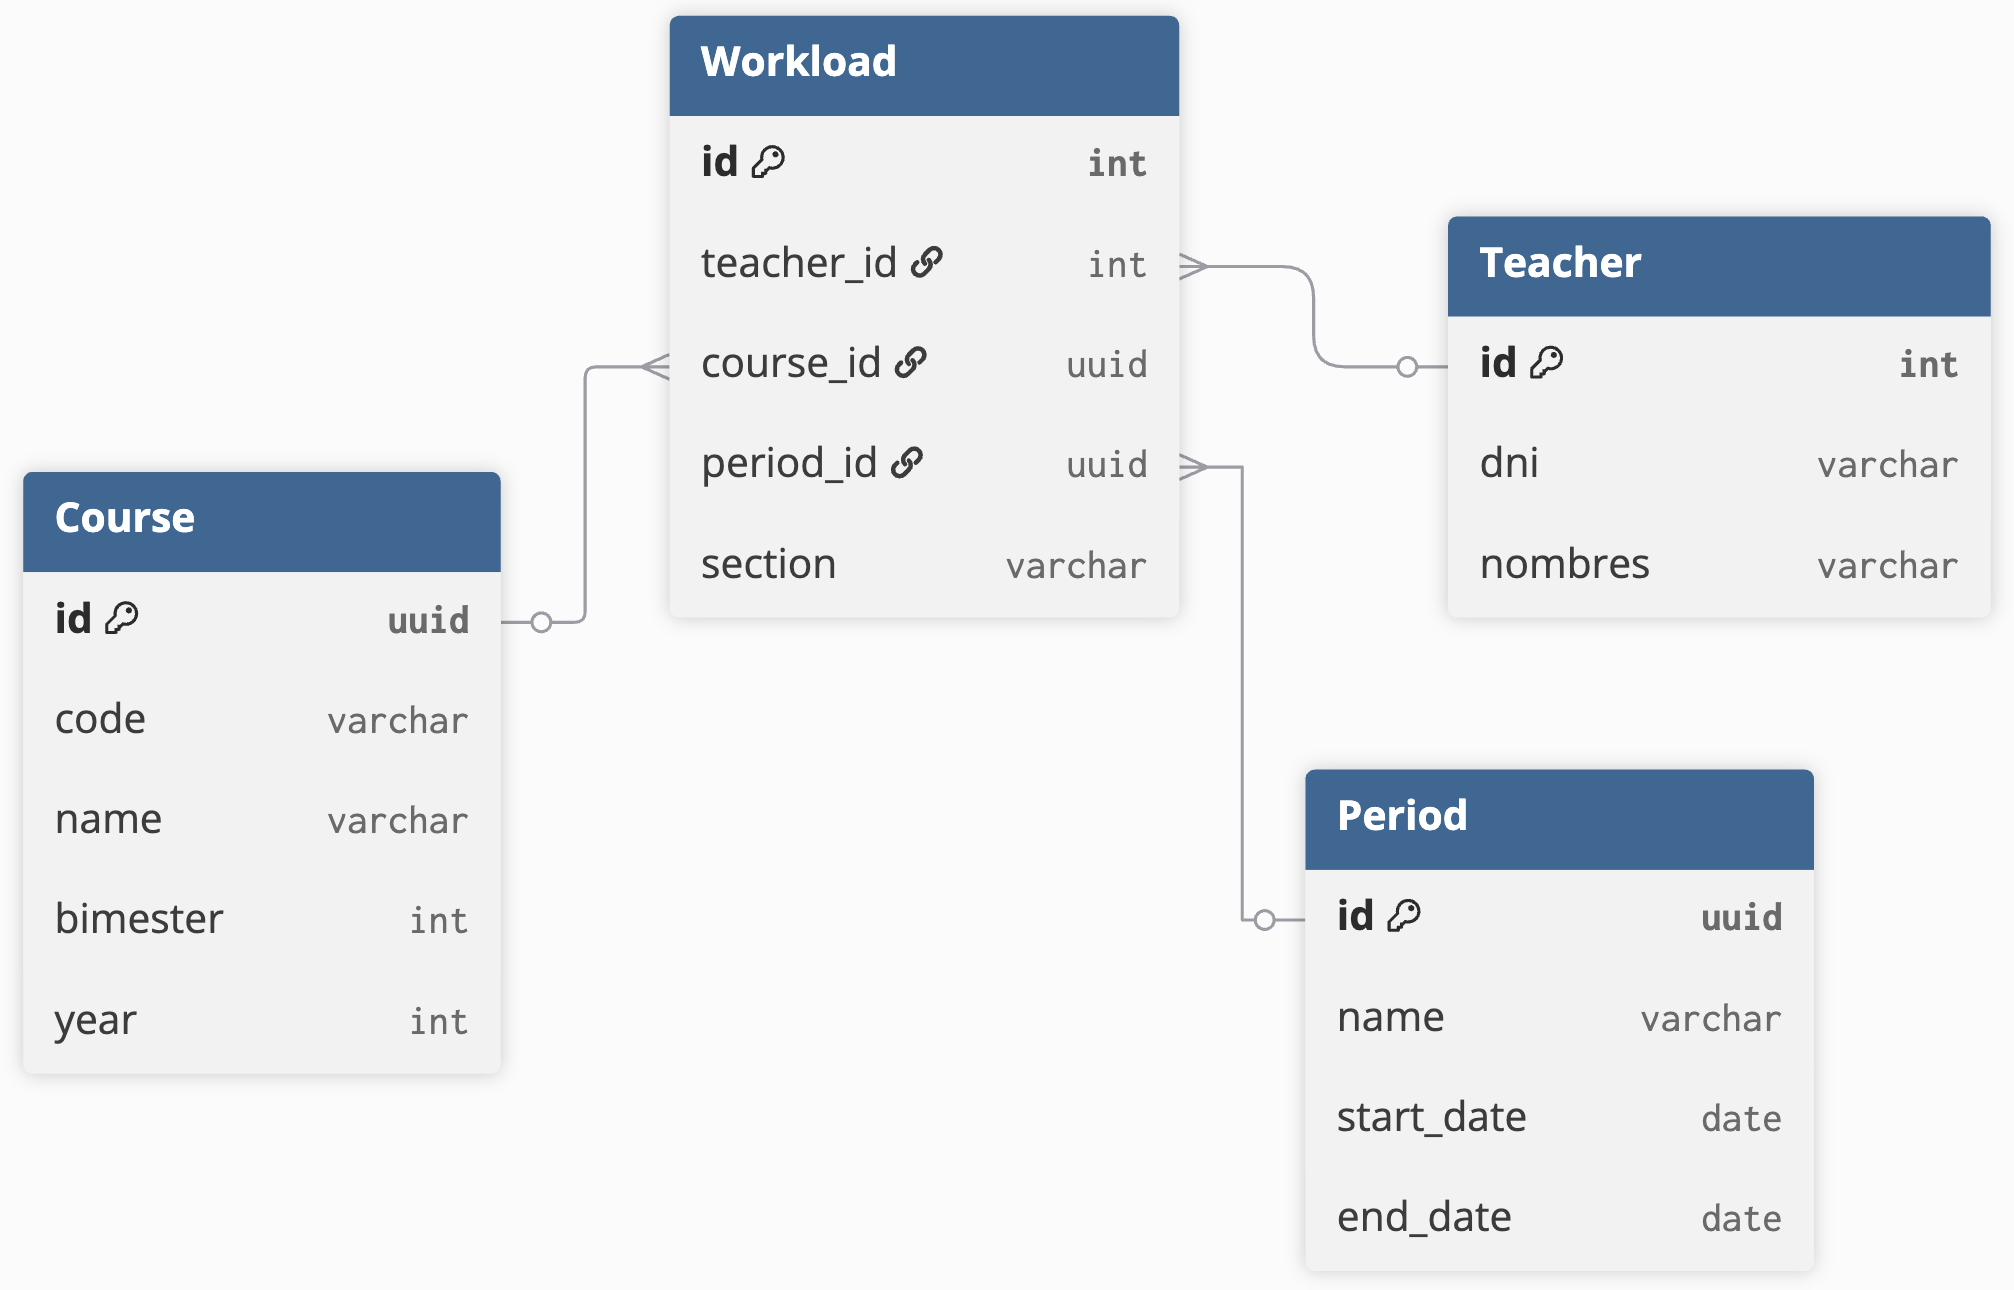
\includegraphics[width=0.7\textwidth]{images/RI1.png}
                \caption{Relaciones entre cursos, docentes, periodos y cargas académicas.}
            \end{figure}
        \subsubsection{Estudiantes, Apoderados e Inscripciones}
            \begin{figure}[H]
                \centering
                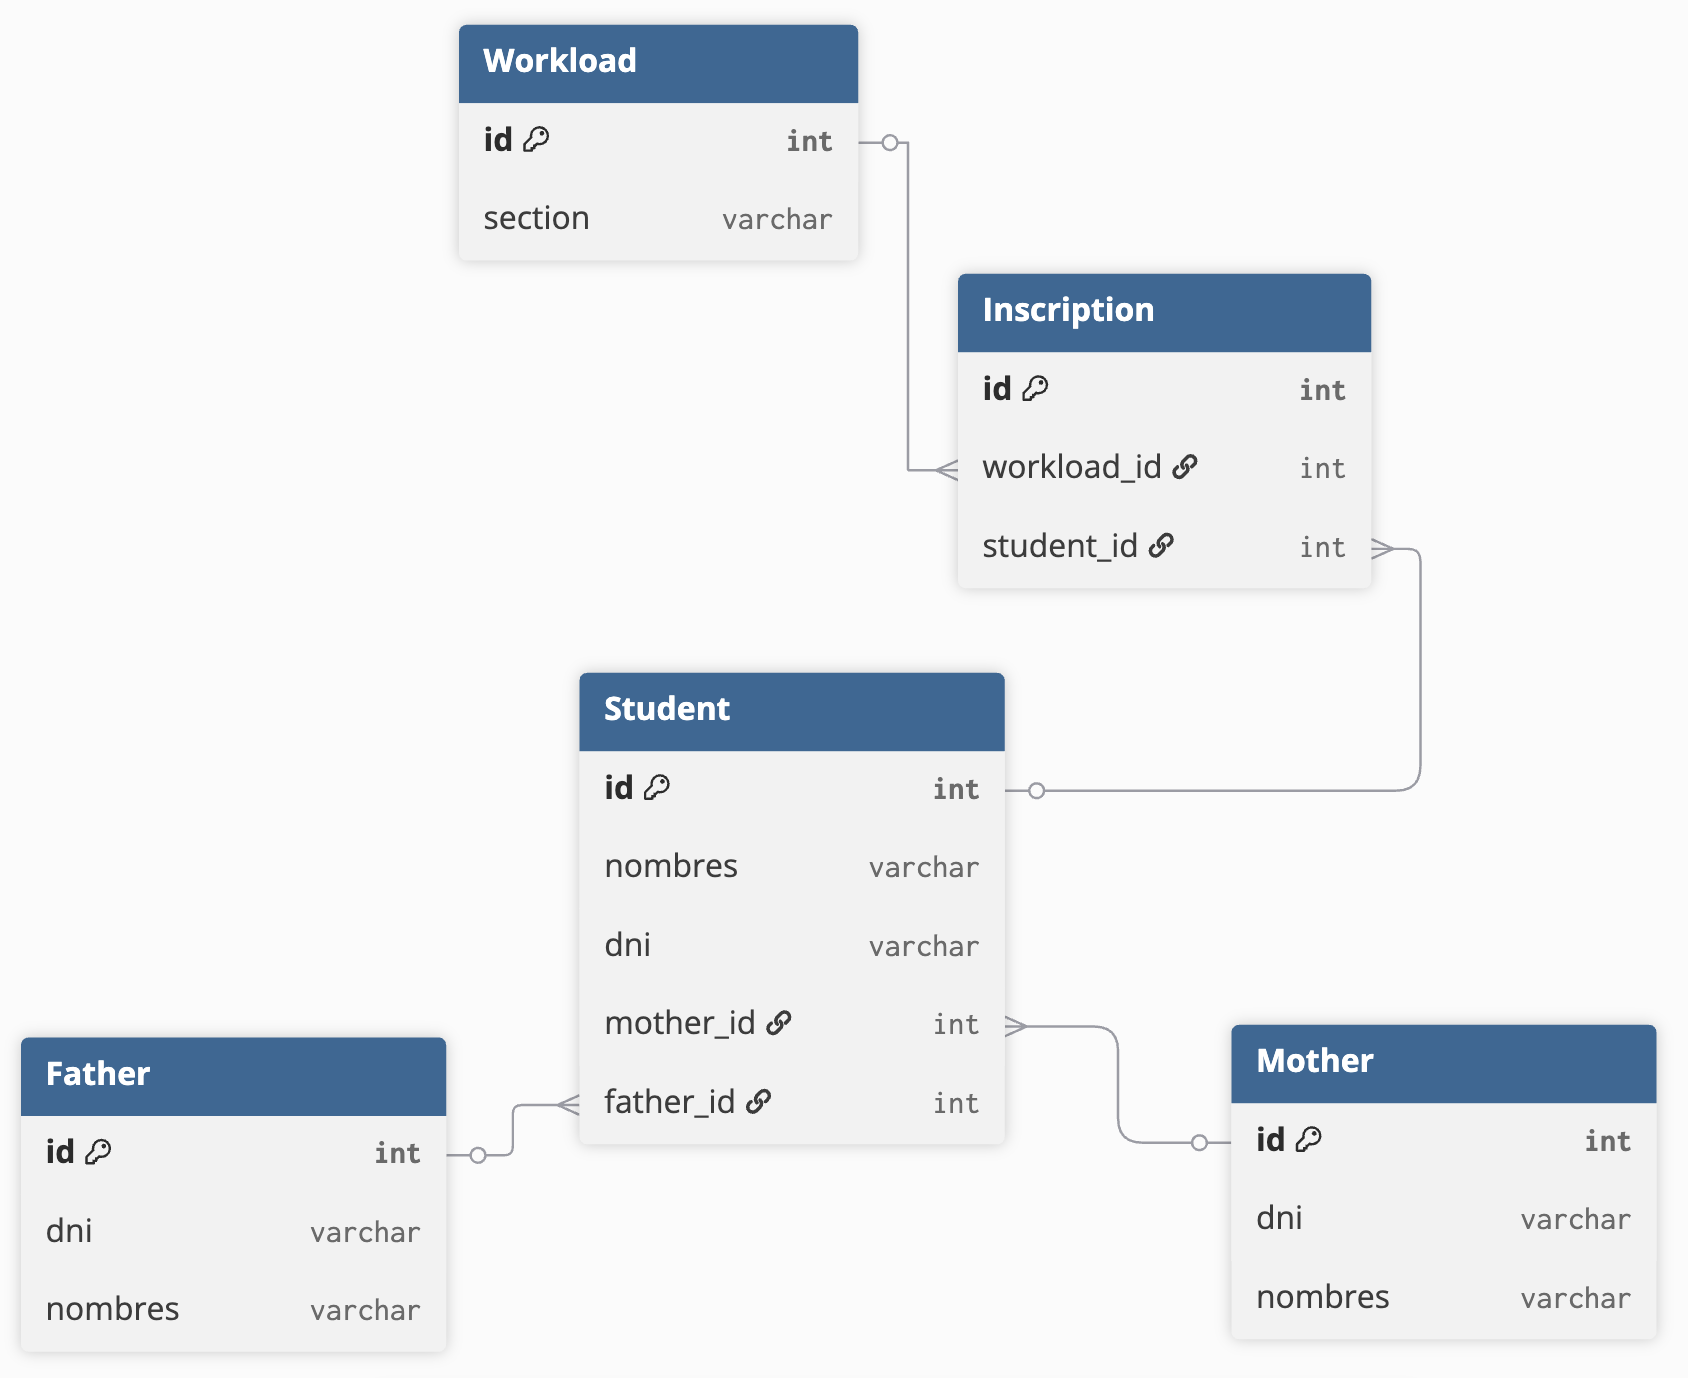
\includegraphics[width=0.7\textwidth]{images/RI2.png}
                \caption{Relaciones entre estudiantes, apoderados e inscripciones.}
            \end{figure}
        \subsubsection{Seguimiento Académico y Recursos}
            \begin{figure}[H]
                \centering
                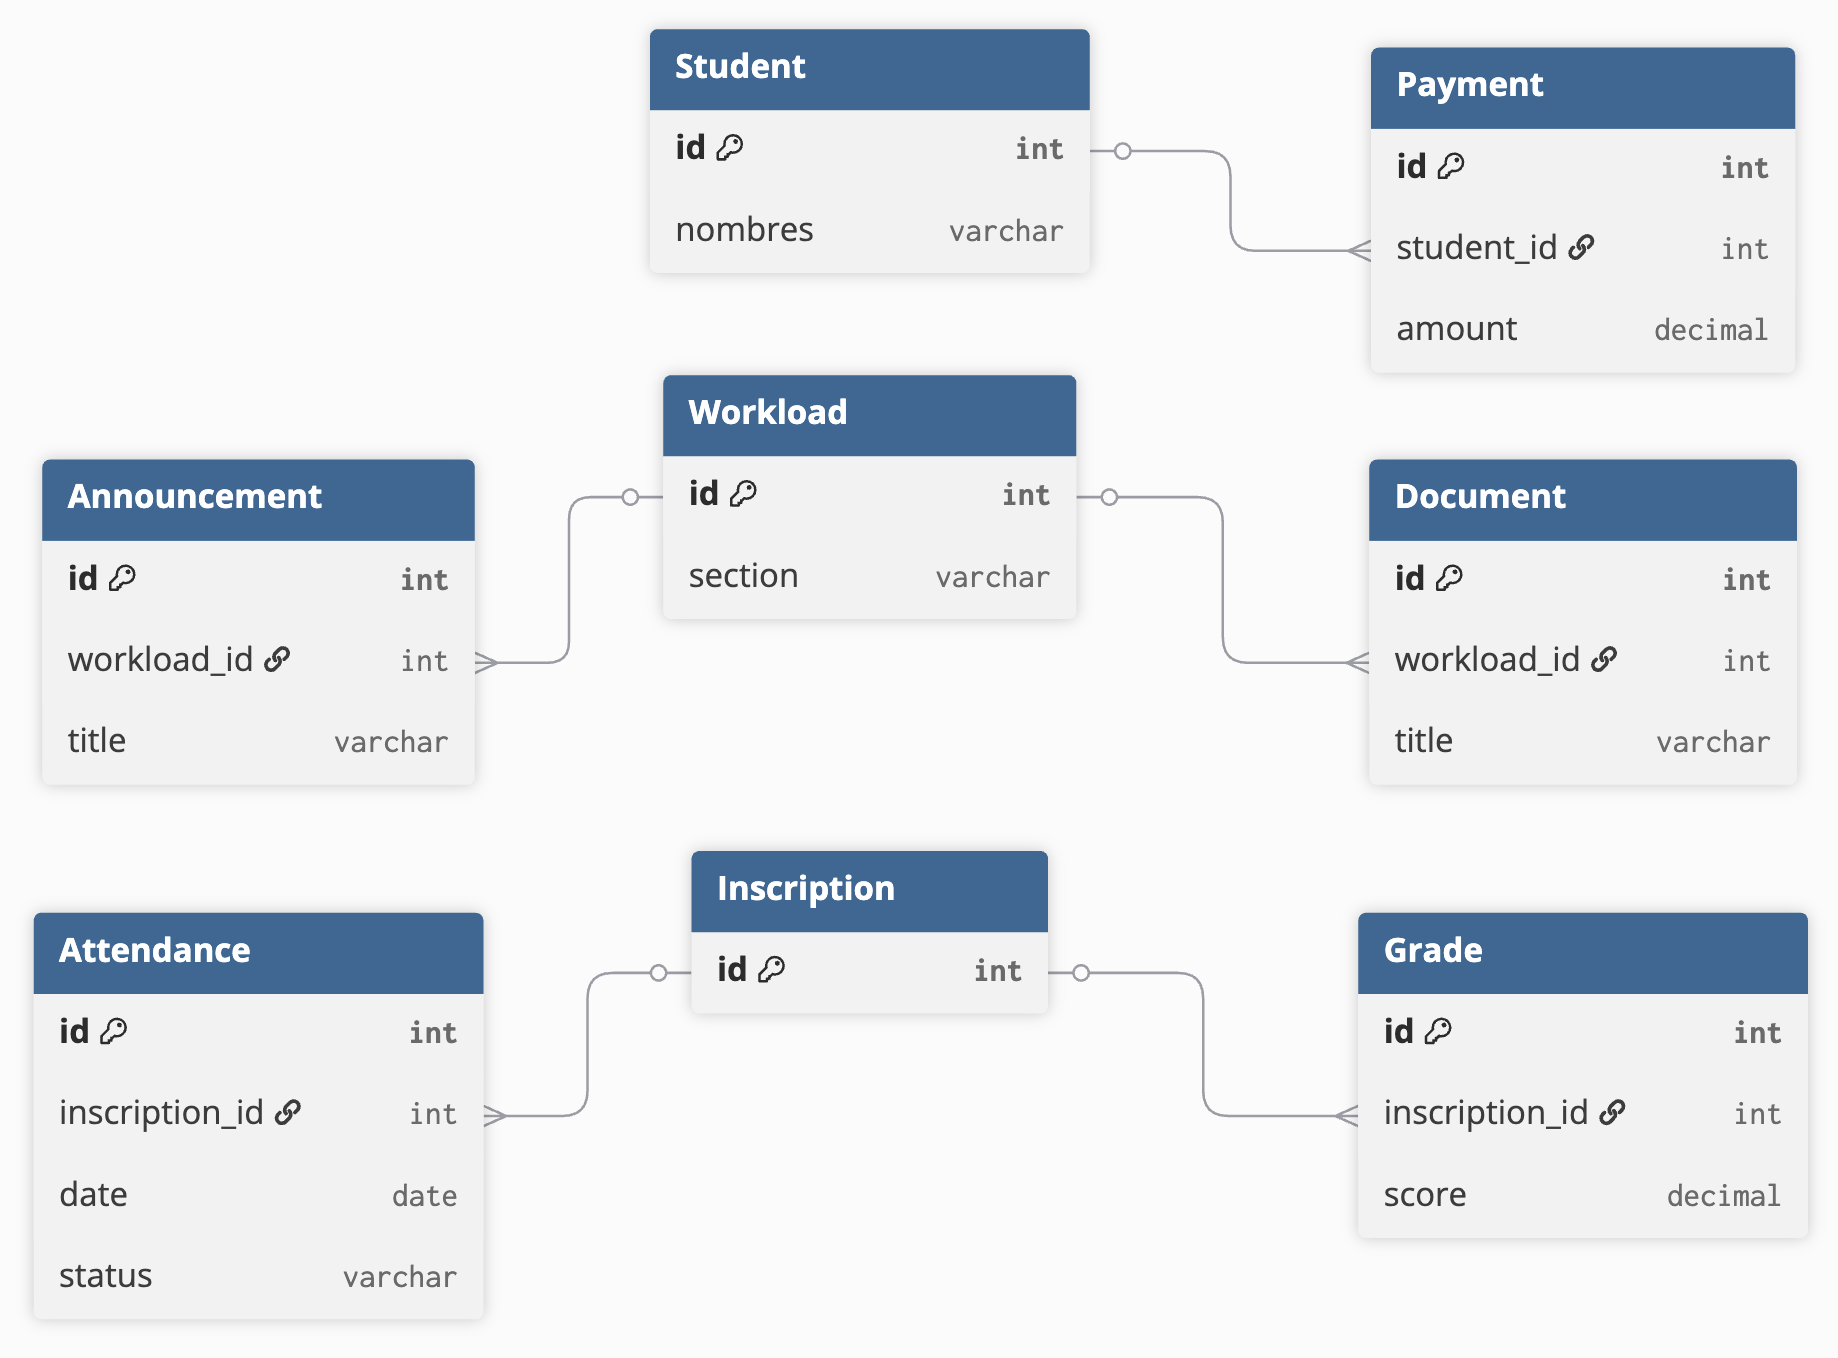
\includegraphics[width=0.7\textwidth]{images/RI3.png}
                \caption{Relaciones para notas, asistencias, pagos y documentos.}
            \end{figure}
    \subsection{Diccionario de Datos}
        En la construcción de software y en el diccionario de datos sobre todo se recomienda y se utilizará el idioma inglés para especificar objetos, atributos, etc.
       
\rowcolors{2}{white}{tabledictionariesbackground!10}
\begin{longtable}{|l|l|l|l|l|l|}
\caption{Course} \\
\hline
\rowcolor{tabledictionariesbackground}
\textbf{Atributo} & \textbf{Tipo} & \textbf{Nulo} & \textbf{Clave} & \textbf{Default} & \textbf{Descripción} \\
\hline
\endfirsthead
\hline
\rowcolor{tabledictionariesbackground}
\textbf{Atributo} & \textbf{Tipo} & \textbf{Nulo} & \textbf{Clave} & \textbf{Default} & \textbf{Descripción} \\
\hline
\endhead
id & UUID & No & PK & auto & Identificador único del curso \\
code & Cadena & Sí & Único & Ninguno & Código institucional \\
name & Cadena & No & No & Ninguno & Nombre del curso \\
credits & Decimal & Sí & No & Ninguno & Créditos académicos \\
bimester & Entero & No & No & 1 & Bimestre donde se dicta \\
year & Entero & No & No & 1 & Año en que se dicta \\
status & Booleano & No & No & True & Activo/Inactivo \\
created & FechaHora & No & No & auto & Fecha de creación \\
modified & FechaHora & No & No & auto & Fecha de modificación \\
\hline
\end{longtable}


\rowcolors{2}{white}{tabledictionariesbackground!10}
\begin{longtable}{|l|l|l|l|l|l|}
\caption{Teacher} \\
\hline
\rowcolor{tabledictionariesbackground}
\textbf{Atributo} & \textbf{Tipo} & \textbf{Nulo} & \textbf{Clave} & \textbf{Default} & \textbf{Descripción} \\
\hline
\endfirsthead

\hline
\rowcolor{tabledictionariesbackground}
\textbf{Atributo} & \textbf{Tipo} & \textbf{Nulo} & \textbf{Clave} & \textbf{Default} & \textbf{Descripción} \\
\hline
\endhead

user & FK (User) & Sí & Único & Null & Usuario vinculado \\
nombres & Cadena & No & No & Ninguno & Nombres del docente \\
apellido\_paterno & Cadena & No & No & Ninguno & Apellido paterno \\
apellido\_materno & Cadena & No & No & Ninguno & Apellido materno \\
dni & Cadena & No & Único & Ninguno & Documento Nacional de Identidad \\
fecha\_nacimiento & Fecha & No & No & Ninguno & Fecha de nacimiento \\
edad & Entero & No & No & Ninguno & Edad actual \\
celular & Cadena & No & No & Ninguno & Número telefónico \\
correo\_personal & Email & No & No & Ninguno & Correo del docente \\
grado\_academico & Cadena & No & No & Licenciado & Nivel académico alcanzado \\
especialidad & Cadena & No & No & Ninguno & Especialidad docente \\
experiencia\_docente & Entero & No & No & 0 & Años de experiencia \\
tipo\_contrato & Cadena & No & No & Contratado & Tipo de contrato laboral \\
facultad & Cadena & No & No & Ninguno & Facultad a la que pertenece \\
escuela\_profesional & Cadena & No & No & Ninguno & Escuela profesional \\
oficina & Cadena & Sí & No & Null & Oficina asignada \\
cv\_documento & Archivo & Sí & No & Null & Archivo PDF del CV \\
activo & Booleano & No & No & True & Estado activo del docente \\
\hline
\end{longtable}



\rowcolors{2}{white}{tabledictionariesbackground!10}
\begin{longtable}{|l|l|l|l|l|l|}
\caption{Student} \\
\hline
\rowcolor{tabledictionariesbackground}
\textbf{Atributo} & \textbf{Tipo} & \textbf{Nulo} & \textbf{Clave} & \textbf{Default} & \textbf{Descripción} \\
\hline
\endfirsthead

\hline
\rowcolor{tabledictionariesbackground}
\textbf{Atributo} & \textbf{Tipo} & \textbf{Nulo} & \textbf{Clave} & \textbf{Default} & \textbf{Descripción} \\
\hline
\endhead

nombres & Cadena & No & No & Ninguno & Nombres del estudiante \\
apellido\_paterno & Cadena & No & No & Ninguno & Apellido paterno \\
apellido\_materno & Cadena & No & No & Ninguno & Apellido materno \\
fecha\_nacimiento & Fecha & No & No & Ninguno & Fecha de nacimiento \\
dni & Cadena & No & Único & Ninguno & Documento Nacional de Identidad \\
sexo & Char & No & No & Ninguno & Sexo biológico (M/F) \\
edad & Entero & No & No & Ninguno & Edad actual \\
lugar\_nacimiento & Cadena & No & No & Ninguno & Lugar de nacimiento \\
domicilio\_actual & Cadena & No & No & Ninguno & Dirección actual \\
limitaciones\_fisicas & Booleano & No & No & False & ¿Tiene limitaciones físicas? \\
especificar\_limitaciones & Texto & Sí & No & Ninguno & Detalles de limitaciones (si aplica) \\
dificultades\_sensoriales & Texto & Sí & No & Ninguno & Dificultades sensoriales \\
alergias & Texto & Sí & No & Ninguno & Alergias conocidas \\
tiene\_seguro\_medico & Booleano & No & No & False & ¿Posee seguro médico? \\
nombre\_seguro\_medico & Cadena & Sí & No & Ninguno & Nombre del seguro \\
mother & FK & Sí & No & Null & Referencia a la madre \\
father & FK & Sí & No & Null & Referencia al padre \\
\hline
\end{longtable}

\rowcolors{2}{white}{tabledictionariesbackground!10}
\begin{longtable}{|l|l|l|l|l|l|}
\caption{Father} \\
\hline
\rowcolor{tabledictionariesbackground}
\textbf{Atributo} & \textbf{Tipo} & \textbf{Nulo} & \textbf{Clave} & \textbf{Default} & \textbf{Descripción} \\
\hline
\endfirsthead
\hline
\rowcolor{tabledictionariesbackground}
\textbf{Atributo} & \textbf{Tipo} & \textbf{Nulo} & \textbf{Clave} & \textbf{Default} & \textbf{Descripción} \\
\hline
\endhead
user & FK (User) & Sí & Único & Null & Usuario vinculado \\
nombres & Cadena & No & No & Ninguno & Nombre de la madre \\
apellido\_paterno & Cadena & No & No & Ninguno & Apellido paterno \\
apellido\_materno & Cadena & No & No & Ninguno & Apellido materno \\
dni & Cadena & No & Único & Ninguno & Documento de identidad \\
edad & Entero & No & No & Ninguno & Edad de la madre \\
fecha\_nacimiento & Fecha & No & No & Ninguno & Fecha de nacimiento \\
celular & Cadena & No & No & Ninguno & Número de contacto \\
correo\_electronico & Email & No & No & Ninguno & Correo institucional \\
estado\_civil & Cadena & No & No & Soltera & Estado civil \\
vive\_con\_el\_nino & Booleano & No & No & True & Vive con el niño \\
grado\_instruccion & Cadena & No & No & secundaria & Nivel educativo \\
ocupacion\_actual & Cadena & No & No & desocupado & Ocupación actual \\
tipo\_dependiente & Cadena & Sí & No & Null & Dependencia laboral \\
rubro\_actividad & Cadena & Sí & No & Null & Actividad económica \\
direccion\_actividad & Texto & Sí & No & Null & Dirección del negocio \\
centro\_estudios & Cadena & Sí & No & Null & Centro de estudios \\
tiene\_vinculo\_unsa & Booleano & No & No & False & Vínculo con la UNSA \\
area\_labora & Cadena & Sí & No & Null & Área donde labora \\
regimen\_laboral & Cadena & Sí & No & Null & Régimen laboral \\
tipo\_docente & Cadena & Sí & No & Null & Tipo de contrato docente \\
tipo\_administrativo & Cadena & Sí & No & Null & Tipo administrativo \\
facultad & Cadena & Sí & No & Null & Facultad asociada \\
escuela & Cadena & Sí & No & Null & Escuela profesional \\
oficina & Cadena & Sí & No & Null & Oficina laboral \\
credentials\_sent & Booleano & No & No & False & ¿Se enviaron credenciales? \\
\hline
\end{longtable}

\rowcolors{2}{white}{tabledictionariesbackground!10}
\begin{longtable}{|l|l|l|l|l|l|}
\caption{Mother} \\
\hline
\rowcolor{tabledictionariesbackground}
\textbf{Atributo} & \textbf{Tipo} & \textbf{Nulo} & \textbf{Clave} & \textbf{Default} & \textbf{Descripción} \\
\hline
\endfirsthead
\hline
\rowcolor{tabledictionariesbackground}
\textbf{Atributo} & \textbf{Tipo} & \textbf{Nulo} & \textbf{Clave} & \textbf{Default} & \textbf{Descripción} \\
\hline
\endhead
user & FK (User) & Sí & Único & Null & Usuario vinculado \\
nombres & Cadena & No & No & Ninguno & Nombre de la madre \\
apellido\_paterno & Cadena & No & No & Ninguno & Apellido paterno \\
apellido\_materno & Cadena & No & No & Ninguno & Apellido materno \\
dni & Cadena & No & Único & Ninguno & Documento de identidad \\
edad & Entero & No & No & Ninguno & Edad de la madre \\
fecha\_nacimiento & Fecha & No & No & Ninguno & Fecha de nacimiento \\
celular & Cadena & No & No & Ninguno & Número de contacto \\
correo\_electronico & Email & No & No & Ninguno & Correo institucional \\
estado\_civil & Cadena & No & No & Soltera & Estado civil \\
vive\_con\_el\_nino & Booleano & No & No & True & Vive con el niño \\
grado\_instruccion & Cadena & No & No & secundaria & Nivel educativo \\
ocupacion\_actual & Cadena & No & No & desocupado & Ocupación actual \\
tipo\_dependiente & Cadena & Sí & No & Null & Dependencia laboral \\
rubro\_actividad & Cadena & Sí & No & Null & Actividad económica \\
direccion\_actividad & Texto & Sí & No & Null & Dirección del negocio \\
centro\_estudios & Cadena & Sí & No & Null & Centro de estudios \\
tiene\_vinculo\_unsa & Booleano & No & No & False & Vínculo con la UNSA \\
area\_labora & Cadena & Sí & No & Null & Área donde labora \\
regimen\_laboral & Cadena & Sí & No & Null & Régimen laboral \\
tipo\_docente & Cadena & Sí & No & Null & Tipo de contrato docente \\
tipo\_administrativo & Cadena & Sí & No & Null & Tipo administrativo \\
facultad & Cadena & Sí & No & Null & Facultad asociada \\
escuela & Cadena & Sí & No & Null & Escuela profesional \\
oficina & Cadena & Sí & No & Null & Oficina laboral \\
credentials\_sent & Booleano & No & No & False & ¿Se enviaron credenciales? \\
\hline
\end{longtable}

\rowcolors{2}{white}{tabledictionariesbackground!10}
\begin{longtable}{|l|l|l|l|l|l|}
\caption{Period} \\
\hline
\rowcolor{tabledictionariesbackground}
\textbf{Atributo} & \textbf{Tipo} & \textbf{Nulo} & \textbf{Clave} & \textbf{Default} & \textbf{Descripción} \\
\hline
\endfirsthead
\hline
\rowcolor{tabledictionariesbackground}
\textbf{Atributo} & \textbf{Tipo} & \textbf{Nulo} & \textbf{Clave} & \textbf{Default} & \textbf{Descripción} \\
\hline
\endhead
id & UUID & No & PK & auto & Identificador único \\
name & Cadena & No & No & Ninguno & Nombre del periodo (Ej: 2025-I) \\
start\_date & Fecha & No & No & Ninguno & Fecha de inicio \\
end\_date & Fecha & No & No & Ninguno & Fecha de fin \\
active & Booleano & No & No & False & ¿Está activo actualmente? \\
\hline
\end{longtable}

\rowcolors{2}{white}{tabledictionariesbackground!10}
\begin{longtable}{|l|l|l|l|l|l|}
\caption{Workload} \\
\hline
\rowcolor{tabledictionariesbackground}
\textbf{Atributo} & \textbf{Tipo} & \textbf{Nulo} & \textbf{Clave} & \textbf{Default} & \textbf{Descripción} \\
\hline
\endfirsthead
\hline
\rowcolor{tabledictionariesbackground}
\textbf{Atributo} & \textbf{Tipo} & \textbf{Nulo} & \textbf{Clave} & \textbf{Default} & \textbf{Descripción} \\
\hline
\endhead
teacher & FK (Teacher) & No & FK & Ninguno & Profesor asignado \\
course & FK (Course) & No & FK & Ninguno & Curso correspondiente \\
period & FK (Period) & No & FK & Ninguno & Periodo académico \\
section & Cadena & No & No & Ninguno & Sección o grupo \\
capacity & Entero & No & No & 30 & Número de vacantes \\
modality & Cadena & No & No & Presencial & Modalidad de enseñanza \\
schedule & Texto & No & No & Ninguno & Horario textual \\
created & FechaHora & No & No & auto & Fecha de creación \\
modified & FechaHora & No & No & auto & Fecha de modificación \\
\hline
\end{longtable}

\rowcolors{2}{white}{tabledictionariesbackground!10}
\begin{longtable}{|l|l|l|l|l|l|}
\caption{Inscription} \\
\hline
\rowcolor{tabledictionariesbackground}
\textbf{Atributo} & \textbf{Tipo} & \textbf{Nulo} & \textbf{Clave} & \textbf{Default} & \textbf{Descripción} \\
\hline
\endfirsthead
\hline
\rowcolor{tabledictionariesbackground}
\textbf{Atributo} & \textbf{Tipo} & \textbf{Nulo} & \textbf{Clave} & \textbf{Default} & \textbf{Descripción} \\
\hline
\endhead
workload & FK (Workload) & No & FK & Ninguno & Carga docente del curso \\
student & FK (Student) & No & FK & Ninguno & Estudiante inscrito \\
status & Booleano & No & No & True & Estado de la inscripción \\
created & FechaHora & No & No & auto & Fecha de inscripción \\
modified & FechaHora & No & No & auto & Fecha de modificación \\
\hline
\end{longtable}

\rowcolors{2}{white}{tabledictionariesbackground!10}
\begin{longtable}{|l|l|l|l|l|l|}
\caption{Grade} \\
\hline
\rowcolor{tabledictionariesbackground}
\textbf{Atributo} & \textbf{Tipo} & \textbf{Nulo} & \textbf{Clave} & \textbf{Default} & \textbf{Descripción} \\
\hline
\endfirsthead
\hline
\rowcolor{tabledictionariesbackground}
\textbf{Atributo} & \textbf{Tipo} & \textbf{Nulo} & \textbf{Clave} & \textbf{Default} & \textbf{Descripción} \\
\hline
\endhead
inscription & FK (Inscription) & No & FK & Ninguno & Inscripción del estudiante \\
evaluation\_type & Cadena & No & No & EXAM & Tipo de evaluación \\
score & Decimal & No & No & Ninguno & Nota obtenida \\
max\_score & Decimal & No & No & 20.00 & Máxima nota posible \\
description & Cadena & Sí & No & Null & Descripción adicional \\
evaluation\_date & Fecha & No & No & Ninguno & Fecha de evaluación \\
weight & Decimal & No & No & 1.00 & Peso de la nota \\
status & Booleano & No & No & True & Estado de la nota \\
created & FechaHora & No & No & auto & Fecha de creación \\
modified & FechaHora & No & No & auto & Fecha de modificación \\
\hline
\end{longtable}

\rowcolors{2}{white}{tabledictionariesbackground!10}
\begin{longtable}{|l|l|l|l|l|l|}
\caption{Payment} \\
\hline
\rowcolor{tabledictionariesbackground}
\textbf{Atributo} & \textbf{Tipo} & \textbf{Nulo} & \textbf{Clave} & \textbf{Default} & \textbf{Descripción} \\
\hline
\endfirsthead
\hline
\rowcolor{tabledictionariesbackground}
\textbf{Atributo} & \textbf{Tipo} & \textbf{Nulo} & \textbf{Clave} & \textbf{Default} & \textbf{Descripción} \\
\hline
\endhead
student & FK (Student) & No & FK & Ninguno & Estudiante que realiza el pago \\
concept & Cadena & No & No & Ninguno & Motivo del pago \\
amount & Decimal & No & No & Ninguno & Monto del pago \\
date & Fecha & No & No & auto & Fecha de pago \\
is\_paid & Booleano & No & No & False & Estado del pago \\
receipt\_number & Cadena & Sí & No & Null & Número de recibo \\
voucher & Archivo & Sí & No & Null & Comprobante escaneado \\
\hline
\end{longtable}

\rowcolors{2}{white}{tabledictionariesbackground!10}
\begin{longtable}{|l|l|l|l|l|l|}
\caption{Document} \\
\hline
\rowcolor{tabledictionariesbackground}
\textbf{Atributo} & \textbf{Tipo} & \textbf{Nulo} & \textbf{Clave} & \textbf{Default} & \textbf{Descripción} \\
\hline
\endfirsthead
\hline
\rowcolor{tabledictionariesbackground}
\textbf{Atributo} & \textbf{Tipo} & \textbf{Nulo} & \textbf{Clave} & \textbf{Default} & \textbf{Descripción} \\
\hline
\endhead
workload & FK (Workload) & No & FK & Ninguno & Curso al que pertenece \\
title & Cadena & No & No & Ninguno & Título del documento \\
description & Texto & Sí & No & Null & Descripción adicional \\
file & Archivo & No & No & Ninguno & Archivo subido \\
uploaded\_at & FechaHora & No & No & auto & Fecha de subida \\
\hline
\end{longtable}

\rowcolors{2}{white}{tabledictionariesbackground!10}
\begin{longtable}{|l|l|l|l|l|l|}
\caption{Chat} \\
\hline
\rowcolor{tabledictionariesbackground}
\textbf{Atributo} & \textbf{Tipo} & \textbf{Nulo} & \textbf{Clave} & \textbf{Default} & \textbf{Descripción} \\
\hline
\endfirsthead
\hline
\rowcolor{tabledictionariesbackground}
\textbf{Atributo} & \textbf{Tipo} & \textbf{Nulo} & \textbf{Clave} & \textbf{Default} & \textbf{Descripción} \\
\hline
\endhead
workload & FK (Workload) & No & FK & Ninguno & Curso al que pertenece \\
sender & FK (User) & No & FK & Ninguno & Usuario que envía el mensaje \\
receiver & FK (User) & No & FK & Ninguno & Usuario que recibe el mensaje \\
message & Texto & No & No & Ninguno & Contenido del mensaje \\
timestamp & FechaHora & No & No & auto & Fecha de envío \\
\hline
\end{longtable}

\rowcolors{2}{white}{tabledictionariesbackground!10}
\begin{longtable}{|l|l|l|l|l|l|}
\caption{Announcement} \\
\hline
\rowcolor{tabledictionariesbackground}
\textbf{Atributo} & \textbf{Tipo} & \textbf{Nulo} & \textbf{Clave} & \textbf{Default} & \textbf{Descripción} \\
\hline
\endfirsthead
\hline
\rowcolor{tabledictionariesbackground}
\textbf{Atributo} & \textbf{Tipo} & \textbf{Nulo} & \textbf{Clave} & \textbf{Default} & \textbf{Descripción} \\
\hline
\endhead
workload & FK (Workload) & No & FK & Ninguno & Curso correspondiente \\
title & Cadena & No & No & Ninguno & Título del anuncio \\
content & Texto & No & No & Ninguno & Cuerpo del anuncio \\
published\_at & FechaHora & No & No & auto & Fecha de publicación \\
\hline
\end{longtable}

\rowcolors{2}{white}{tabledictionariesbackground!10}
\begin{longtable}{|l|l|l|l|l|l|}
\caption{Attendance} \\
\hline
\rowcolor{tabledictionariesbackground}
\textbf{Atributo} & \textbf{Tipo} & \textbf{Nulo} & \textbf{Clave} & \textbf{Default} & \textbf{Descripción} \\
\hline
\endfirsthead
\hline
\rowcolor{tabledictionariesbackground}
\textbf{Atributo} & \textbf{Tipo} & \textbf{Nulo} & \textbf{Clave} & \textbf{Default} & \textbf{Descripción} \\
\hline
\endhead
inscription & FK (Inscription) & No & FK & Ninguno & Inscripción asociada \\
date & Fecha & No & No & Ninguno & Fecha de asistencia \\
status & Cadena & No & No & Ninguno & Presente, Ausente o Tardanza \\
\hline
\end{longtable}




\section{Implementación del Backend}
    \subsection{Creación del Proyecto y Aplicaciones en Django}
        \begin{itemize}
            \item El desarrollo del backend comenzó con la creación del proyecto principal de Django utilizando el comando:
            \item Posteriormente, se generó la aplicación base del sistema denominada \texttt{AppCuna}, mediante el siguiente comando:
        \end{itemize}
        \begin{lstlisting}[language=bash, caption={Creación del Proyecto Django}, numbers=none]
        $ django-admin startproject MyDjangoProject
        \end{lstlisting}
        \begin{lstlisting}[language=bash, caption={Creación de la aplicación AppCuna}, numbers=none]
        $ python manage.py startapp AppCuna
        \end{lstlisting}

        A continuación, se registró la aplicación en el archivo \texttt{settings.py} dentro del arreglo \texttt{INSTALLED\_APPS}, junto con otros módulos requeridos como \texttt{rest\_framework} para la gestión de APIs.
    \subsection{Modelos y Migraciones}
    \begin{itemize}
        \item Los modelos fueron definidos dentro del archivo \texttt{models/} de la aplicación \texttt{AppCuna}, cada uno representando una entidad del dominio del sistema: estudiantes, docentes, cursos, periodos, inscripciones, pagos, entre otros.
        \item Una vez definidos los modelos, se ejecutaron los siguientes comandos para generar y aplicar las migraciones a la base de datos:

    \end{itemize}


\begin{lstlisting}[language=bash, caption={Migraciones de los modelos}, numbers=none]
        $ python manage.py makemigrations
        $ python manage.py migrate
\end{lstlisting}

Estas operaciones crearon las tablas correspondientes en la base de datos PostgreSQL, las cuales fueron validadas mediante inspección directa y pruebas funcionales iniciales.


    \subsection{Panel de Administración}
        \begin{itemize}
            \item Django proporciona un panel administrativo integrado, el cual fue configurado para gestionar de manera visual las entidades del sistema.
            \item Para ello, se registraron los modelos relevantes en el archivo \texttt{admin.py} de \texttt{AppCuna} mediante el decorador \texttt{@admin.register}, o utilizando la función \texttt{admin.site.register()}.
            \item Se creó un superusuario ejecutando el siguiente comando:
        \end{itemize}
        \begin{lstlisting}[language=bash, caption={Creación del superusuario}, numbers=none]
        $ python manage.py createsuperuser
        \end{lstlisting}

        El panel de administración permite crear, editar, eliminar y buscar registros de estudiantes, docentes, cursos, inscripciones, notas, pagos y asistencia, facilitando la gestión inicial del sistema mientras se desarrollan las interfaces de usuario en el frontend.
    
    \subsection{Migración a PostgreSQL y Conexión con Supabase}
        \begin{itemize}
            \item Inicialmente, el sistema utilizaba \texttt{SQLite} como base de datos por defecto para pruebas locales. Para el entorno de producción, se realizó una migración a \textbf{PostgreSQL}, aprovechando los servicios en la nube de \textbf{Supabase}, que ofrece una instancia segura, escalable y de alto rendimiento.
            \item Para conectar con Supabase, se implementó la siguiente lógica en el archivo \texttt{settings.py}, utilizando variables de entorno y la biblioteca \texttt{dj\_database\_url}:
        \end{itemize}

        \begin{lstlisting}[language=Python, caption={Configuración de la base de datos con Supabase}]
if 'DATABASE_URL' in os.environ:
    DATABASES = {
        'default': dj_database_url.parse(os.getenv('DATABASE_URL'))
    }
else:
    DATABASES = {
        'default': {
            'ENGINE': 'django.db.backends.postgresql',
            'NAME': os.getenv('DB_NAME', 'postgres'),
            'USER': os.getenv('DB_USER', 'postgres.zcsblgjwreggdewwdyxf'),
            'PASSWORD': os.getenv('DB_PASSWORD', 'CunaUnsa-'),
            'HOST': os.getenv('DB_HOST', 'aws-0-us-east-2.pooler.supabase.com'),
            'PORT': os.getenv('DB_PORT', '6543'),
            'OPTIONS': {
                'sslmode': 'require',
            }
        }
    }
        \end{lstlisting}
        \begin{itemize}
            \item Para activar esta conexión, se definieron las variables de entorno correspondientes en el archivo \texttt{.env} o mediante configuración del servidor en producción. También se instaló la dependencia necesaria:
            \item Una vez configurado todo, se ejecutaron las migraciones de los modelos con el comando:
        \end{itemize}

        \begin{lstlisting}[language=bash, caption={Instalación de dependencias}, numbers=none]
        $ pip install dj-database-url psycopg2-binary
        \end{lstlisting}

        \begin{lstlisting}[language=bash, caption={Ejecucion de migraciones}, numbers=none]
        $ python manage.py migrate
        \end{lstlisting}

        Esta configuración permite una conexión segura (SSL) y flexible entre Django y Supabase, facilitando tanto el desarrollo como el despliegue de la aplicación en la nube.

    %%%%%%%%%%%%%%%%%%%%%%%%%%%%%%%%%%%%%%%%%%%%%%%%%%%%%%%
    \subsection{Serializers y Vistas (DRF)}
    \subsubsection*{Instalación y configuración}
    \begin{itemize}
        \item Para construir la API REST del backend se utilizó el paquete \textbf{Django REST Framework (DRF)}. Este framework permite crear endpoints robustos para modelos, aplicar validaciones personalizadas, gestionar permisos por rol y adaptar la respuesta según el usuario autenticado. DRF fue instalado mediante el siguiente comando:
        \item Luego, se añadió a \texttt{INSTALLED\_APPS}:
    \end{itemize}
    \begin{lstlisting}[language=bash, caption={Instalación de Django REST Framework}, numbers=none]
        $ pip install djangorestframework
    \end{lstlisting}



\begin{lstlisting}[language=Python, caption={Agregar DRF al proyecto}, numbers=none]
INSTALLED_APPS = [
    ...,
    'rest_framework',
]
\end{lstlisting}

\subsubsection*{Serializers y vistas destacadas}

A continuación, se describen tres serializers clave del sistema y sus vistas asociadas.

\paragraph{1. StudentSerializer y StudentViewSet}

Este serializer impone restricciones dinámicas según el rol del usuario. Por ejemplo, un padre o madre autenticado solo puede editar campos específicos de su hijo.

\begin{lstlisting}[language=Python, caption={StudentSerializer simplificado}]
class StudentSerializer(serializers.ModelSerializer):
    def __init__(self, *args, **kwargs):
        super().__init__(*args, **kwargs)
        request = self.context.get('request')
        if request and request.user.is_authenticated:
            is_parent = (Father.objects.filter(user=request.user).exists() or 
                         Mother.objects.filter(user=request.user).exists())
            if is_parent:
                for field in ['dni', 'fecha_nacimiento', 'sexo']:
                    self.fields[field].read_only = True

    class Meta:
        model = Student
        fields = '__all__'
\end{lstlisting}

La vista asociada filtra los estudiantes según el rol:

\begin{lstlisting}[language=Python, caption={StudentViewSet resumido}]
class StudentViewSet(viewsets.ModelViewSet):
    queryset = Student.objects.all()
    serializer_class = StudentSerializer

    def get_queryset(self):
        user = self.request.user
        if user.is_superuser:
            return Student.objects.all()
        try:
            teacher = Teacher.objects.get(user=user)
            workloads = Workload.objects.filter(teacher=teacher)
            inscriptions = Inscription.objects.filter(workload__in=workloads)
            return Student.objects.filter(inscription__in=inscriptions).distinct()
        except:
            ...
\end{lstlisting}

\paragraph{2. GradeSerializer y GradeViewSet}

Este serializer filtra las inscripciones disponibles según el docente autenticado:

\begin{lstlisting}[language=Python, caption={GradeSerializer filtrando inscripciones}]
class GradeSerializer(serializers.ModelSerializer):
    def __init__(self, *args, **kwargs):
        super().__init__(*args, **kwargs)
        request = self.context.get('request')
        if request and request.user.is_authenticated:
            try:
                teacher = Teacher.objects.get(user=request.user)
                teacher_workloads = Workload.objects.filter(teacher=teacher)
                self.fields['inscription'].queryset = Inscription.objects.filter(
                    workload__in=teacher_workloads
                )
            except:
                ...
    class Meta:
        model = Grade
        fields = '__all__'
\end{lstlisting}

\paragraph{3. AnnouncementSerializer y AnnouncementViewSet}

Este serializer limita los workloads al docente correspondiente:

\begin{lstlisting}[language=Python, caption={AnnouncementSerializer con filtrado}]
class AnnouncementSerializer(serializers.ModelSerializer):
    def __init__(self, *args, **kwargs):
        super().__init__(*args, **kwargs)
        request = self.context.get('request')
        if request and request.user.is_authenticated:
            try:
                teacher = Teacher.objects.get(user=request.user)
                self.fields['workload'].queryset = Workload.objects.filter(teacher=teacher)
            except:
                ...
    class Meta:
        model = Announcement
        fields = '__all__'
\end{lstlisting}

    \subsection{URLs y Rutas}

La configuración de rutas del proyecto permite acceder a todos los endpoints del backend mediante un sistema jerárquico organizado en dos niveles:

\begin{itemize}
    \item El archivo \texttt{urls.py} principal del proyecto redirige desde la raíz hacia el prefijo \texttt{/api/}.
    \item El archivo \texttt{AppCuna/urls.py} registra todas las rutas de la aplicación utilizando el router de Django REST Framework y también define rutas personalizadas para autenticación.
\end{itemize}

A continuación se muestra el contenido de cada archivo clave.

\begin{lstlisting}[language=Python, caption={Archivo MyDjangoProject/urls.py}]
from django.contrib import admin
from django.urls import path, include
from django.shortcuts import redirect

def redirect_to_api(request):
    return redirect('/api/')

urlpatterns = [
    path('admin/', admin.site.urls),
    path('api/', include('AppCuna.urls')),
    path('', redirect_to_api),  
]
\end{lstlisting}

Este archivo configura dos rutas principales:
\begin{itemize}
    \item \texttt{/admin/}: Panel administrativo de Django.
    \item \texttt{/api/}: Redirecciona al módulo de rutas de la aplicación \texttt{AppCuna}.
\end{itemize}

\begin{lstlisting}[language=Python, caption={Archivo AppCuna/urls.py}]
from django.urls import path, include
from rest_framework.routers import DefaultRouter
from .views import *

router = DefaultRouter()
router.register(r'students', StudentViewSet)
router.register(r'padres', FatherViewSet)
router.register(r'madres', MotherViewSet)
router.register(r'teachers', TeacherViewSet)
router.register(r'workloads', WorkloadViewSet)
router.register(r'courses', CourseViewSet)
router.register(r'inscriptions', InscriptionViewSet)
router.register(r'grades', GradeViewSet)
router.register(r'payments', PaymentViewSet)
router.register(r'announcements', AnnouncementViewSet)
router.register(r'attendance', AttendanceViewSet)
router.register(r'periods', PeriodViewSet)
router.register(r'chats', ChatViewSet)
router.register(r'documents', DocumentViewSet)

urlpatterns = [
    path('', include(router.urls)),

    path('auth/register/father/', RegisterFatherAPIView.as_view(), name='register-father'),
    path('auth/register/mother/', RegisterMotherAPIView.as_view(), name='register-mother'),
    path('auth/register/teachers/', RegisterTeacherAPIView.as_view(), name='register-teacher'),
    path('auth/login/', LoginAPIView.as_view(), name='login'),
    path('auth/logout/', LogoutAPIView.as_view(), name='logout'),
    path('auth/profile/', ProfileAPIView.as_view(), name='profile'),
    path('auth/credentials/', GetCredentialsAPIView.as_view(), name='get-credentials'),

    # Admin tokens
    path('auth/get-token/', GetUserTokenAPIView.as_view(), name='get-token'),
    path('auth/all-tokens/', GetAllTokensAPIView.as_view(), name='all-tokens'),
]
\end{lstlisting}

\subsubsection*{Estructura General de Endpoints}

Los endpoints generados automáticamente por el router se resumen en la siguiente tabla:

\begin{table}[ht]
\centering
\begin{tabular}{|l|l|}
\hline
\rowcolor{tabledictionariesbackground!30}
\textbf{Endpoint} & \textbf{Descripción} \\
\hline
\texttt{/api/students/} & Gestión de estudiantes \\
\texttt{/api/padres/} & Gestión de padres \\
\texttt{/api/madres/} & Gestión de madres \\
\texttt{/api/teachers/} & Gestión de docentes \\
\texttt{/api/workloads/} & Gestión de asignaciones docentes \\
\texttt{/api/courses/} & Gestión de cursos \\
\texttt{/api/inscriptions/} & Inscripciones de estudiantes a cursos \\
\texttt{/api/grades/} & Notas por inscripción \\
\texttt{/api/payments/} & Pagos de matrícula u otros \\
\texttt{/api/announcements/} & Anuncios por parte de docentes \\
\texttt{/api/attendance/} & Asistencia de estudiantes \\
\texttt{/api/periods/} & Periodos académicos \\
\texttt{/api/chats/} & Mensajes en el sistema \\
\texttt{/api/documents/} & Documentos institucionales \\
\hline
\end{tabular}
\caption{Principales endpoints generados por DRF Router}
\end{table}

    %%%%%%%%%%%%%%%%%%%%%%%%%%%%%%%%%%%%%%%%%%%%%%%%%%%%%%%%
    \subsection{Autenticación con Tokens}

El sistema implementa autenticación dual: mediante sesiones de Django (para navegación en navegador) y mediante tokens JWT (para consumo desde herramientas como Postman o aplicaciones frontend como Angular). Esta combinación permite flexibilidad tanto en pruebas como en producción.

\subsubsection*{Configuración en \texttt{settings.py}}

Se activan ambas clases de autenticación en el backend mediante:

\begin{lstlisting}[language=Python, caption={Configuración de autenticación en settings.py}]
REST_FRAMEWORK = {
    'DEFAULT_AUTHENTICATION_CLASSES': [
        'rest_framework_simplejwt.authentication.JWTAuthentication',
        'rest_framework.authentication.SessionAuthentication',
    ],
    'DEFAULT_PERMISSION_CLASSES': [
        'rest_framework.permissions.IsAuthenticated',
    ],
    ...
}
\end{lstlisting}

\subsubsection*{Login con Tokens}

El login se realiza vía el endpoint:

\begin{itemize}
  \item \texttt{POST /api/auth/login/}
\end{itemize}

Este endpoint procesa credenciales (DNI y contraseña) mediante el \texttt{LoginAPIView}. Si son válidas, se activa automáticamente una sesión del lado del navegador y además se generan tokens JWT:

\begin{lstlisting}[language=Python, caption={Respuesta JSON al hacer login}]
{
  "success": true,
  "tokens": {
    "access": "eyJ0eXAiOiJKV1QiLCJh...",
    "refresh": "eyJ0eXAiOiJKV1QiLCJhbGci..."
  },
  "user_type": "father",
  "user_data": { ... }
}
\end{lstlisting}

\subsubsection*{Logout y Perfil}

El sistema permite cerrar la sesión y consultar los datos del usuario autenticado:

\begin{itemize}
  \item \texttt{POST /api/auth/logout/} – cierra la sesión activa.
  \item \texttt{GET /api/auth/profile/} – devuelve información útil y enlaces según el rol (padre, madre, docente o admin).
\end{itemize}

\subsubsection*{Rutas para desarrollo (tokens de prueba)}

Para facilitar pruebas, se habilitan rutas protegidas para desarrollo:

\begin{itemize}
  \item \texttt{POST /api/auth/get-token/}: permite obtener un token JWT ingresando solo el DNI.
  \item \texttt{GET /api/auth/all-tokens/}: lista todos los usuarios registrados con sus respectivos tokens.
\end{itemize}

Estas rutas están marcadas en la documentación con advertencias y no deben usarse en entornos de producción.

\subsubsection*{Autenticación desde herramientas externas}

Una vez obtenido el \texttt{access token}, puede utilizarse en herramientas como Postman, Insomnia o desde Vue, enviándolo en el encabezado HTTP:

\begin{lstlisting}[language=bash, caption={Ejemplo de uso con curl}]
curl -H "Authorization: Bearer <ACCESS_TOKEN>" http://localhost:8000/api/grades/
\end{lstlisting}

\subsubsection*{Resumen de Endpoints de Autenticación}

\begin{table}[H]
\centering
\begin{tabular}{|p{5cm}|p{9cm}|}
\hline
\rowcolor{tabledictionariesbackground!30}
\textbf{Ruta} & \textbf{Descripción} \\
\hline
\texttt{POST /api/auth/login/} & Inicia sesión y retorna tokens JWT + sesión \\
\texttt{POST /api/auth/logout/} & Cierra la sesión activa \\
\texttt{GET /api/auth/profile/} & Devuelve datos del usuario autenticado y opciones según rol \\
\texttt{POST /api/auth/get-token/} & (Dev) Genera tokens ingresando el DNI \\
\texttt{GET /api/auth/all-tokens/} & (Dev) Lista todos los usuarios con sus tokens \\
\hline
\end{tabular}
\caption{Rutas principales del sistema de autenticación}
\end{table}



     %%%%%%%%%%%%%%%%%%%%%%%%%%%%%%%%%%%%%%%%%%%%%%%%%%%%%%%%


\section{Implementación desl Frontend}
    \subsection{Creación del Proyecto Vue}

        Para desarrollar la interfaz de usuario del sistema, se utilizó Vue 3, un framework progresivo para la construcción de interfaces web. El proyecto fue creado utilizando la herramienta oficial de línea de comandos \texttt{@vue/cli}. A continuación, se detallan los archivos clave relacionados con la creación y configuración del proyecto.

        \begin{lstlisting}[language=bash, caption={package.json - Configuración del Proyecto}]
{
"name": "cuna-frontend",
"version": "1.0.0",
"private": true,
"scripts": {
    "serve": "vue-cli-service serve",
    "build": "vue-cli-service build",
    "lint": "vue-cli-service lint"
    },
"dependencies": {
    "@fortawesome/fontawesome-free": "^7.0.0",
    "axios": "^1.6.0",
    "bootstrap": "^5.3.0",
    "core-js": "^3.8.3",
    "vue": "^3.2.13",
    "vue-router": "^4.0.3",
    "vuex": "^4.0.0"
    }
}
        \end{lstlisting}

        El archivo \texttt{package.json} define las dependencias principales del proyecto, como Vue, Vuex, Vue Router, Bootstrap y Axios. También incluye scripts útiles como \texttt{serve} para iniciar el servidor de desarrollo local y \texttt{build} para generar la versión optimizada del sitio.

        \begin{lstlisting}[language=bash, caption={vue.config.js - Proxy de Desarrollo}]
module.exports = {
    publicPath: '/',
    outputDir: 'dist',
    assetsDir: 'assets',
        devServer: {
            proxy: {
            '/api': {
                target: 'https://cuna-unsa-production.up.railway.app',
                changeOrigin: true,
                secure: true,
                }
            }
        }
}
        \end{lstlisting}

        El archivo \texttt{vue.config.js} permite definir opciones de compilación y desarrollo. En este caso, se configura un proxy que redirige automáticamente las solicitudes a \texttt{/api} hacia el backend desplegado en Railway, lo cual facilita las pruebas sin problemas de CORS durante el desarrollo local.

    \subsection{Componentes y Servicios}
        En el desarrollo del frontend con Vue.js, se estructuraron los distintos elementos visuales y de interaccion del sistema a traves de componentes reutilizables y servicios de conexion con la API. A continuacion, se describe la logica de algunos componentes clave.

        \subsubsection*{Componente de Login}

        El archivo \texttt{Login.vue} contiene el formulario de autenticacion que permite a los usuarios ingresar al sistema. Utiliza \texttt{v-model} para enlazar datos con los campos del formulario y acciones de Vuex para despachar la operacion de login. 

        \begin{lstlisting}[language=HTML, caption={Formulario de Login (Login.vue)}]
<form @submit.prevent="handleLogin">
<input v-model="form.username" required />
<input v-model="form.password" type="password" required />
<button type="submit" :disabled="loading">
    {{ loading ? 'Iniciando...' : 'Iniciar Sesion' }}
</button>
</form>
        \end{lstlisting}

        En la seccion de metodos se utiliza una accion del store para realizar la peticion de autenticacion al backend:

        \begin{lstlisting}[language=bash, caption={Logica de Login}]
methods: {
...mapActions(['login']),
async handleLogin() {
    try {
    const res = await this.login(this.form)
    this.$router.push('/dashboard')
    } catch (error) {
    console.error('Error en login:', error)
    }
}
}
        \end{lstlisting}

        \subsubsection*{Vista Principal: Dashboard}

        El componente \texttt{Dashboard.vue} representa el panel principal al que se redirige luego del login. En esta vista se integran otros componentes secundarios y datos obtenidos desde la API. Aunque su logica es sencilla, sirve como punto de partida para acceder a distintas secciones como cursos, estudiantes o calificaciones.

        \subsubsection*{Componente Comun: Barra de Navegacion}

        En la carpeta \texttt{components/common/} se implemento una barra de navegacion dinamica que muestra diferentes enlaces segun el estado de autenticacion del usuario. Utiliza \texttt{router-link} para la navegacion y datos provenientes del \texttt{store} para personalizar la interfaz.

        \begin{lstlisting}[language=HTML, caption={Fragmento de Navbar.vue}]
<router-link class="nav-link" to="/dashboard">Pagina Principal</router-link>
<router-link class="nav-link" to="/grades">Calificaciones</router-link>
<a class="dropdown-item text-danger" href="#" @click="handleLogout">
Cerrar Sesion
</a>
        \end{lstlisting}

        \subsubsection*{Servicios de Conexion}

        El archivo \texttt{services/api.js} contiene la instancia de Axios configurada para conectarse con el backend desplegado, permitiendo que todos los componentes puedan acceder a los datos protegidos mediante un proxy local durante el desarrollo.

        \begin{lstlisting}[language=bash, caption={Instancia de Axios}]
import axios from 'axios'

const api = axios.create({
baseURL: '/api',
timeout: 5000
})

export default api
        \end{lstlisting}
%%%%%%%

\subsection{Conexión a la API REST}

Para establecer la comunicación entre el cliente (Vue.js) y el servidor backend (Django + DRF), se creó un archivo \texttt{api.js} dentro del directorio \texttt{src/services/}. Este módulo configura la librería \texttt{Axios} para realizar solicitudes HTTP con autenticación mediante tokens.

\begin{itemize}
  \item Se define una instancia de \texttt{Axios} con la URL base tomada desde una variable de entorno (\texttt{VUE\_APP\_API\_URL}).
  \item Se usan interceptores para incluir el token de autenticación almacenado en \texttt{localStorage} en cada solicitud.
  \item Ante errores de autenticación (\texttt{401 Unauthorized}), el sistema elimina el token y redirige automáticamente al login.
  \item Las rutas implementadas permiten operaciones completas (GET, POST, PUT, DELETE) sobre entidades como estudiantes, docentes y cursos.
\end{itemize}

\begin{lstlisting}[language=bash, caption={Ejemplo de configuración de Axios en api.js}]
const apiInstance = axios.create({
  baseURL: process.env.VUE_APP_API_URL,
  headers: {
    'Content-Type': 'application/json',
  },
  timeout: 10000,
  withCredentials: true,
});

apiInstance.interceptors.request.use((config) => {
  const token = localStorage.getItem('token');
  if (token) {
    config.headers.Authorization = `Bearer ${token}`;
  }
  return config;
});
\end{lstlisting}

\textbf{Ejemplo de consumo en un componente:} el método \texttt{login} desde la vista \texttt{Login.vue} invoca \texttt{api.login()} usando datos del formulario.

\begin{lstlisting}[language=bash, caption={Invocación del login}]
methods: {
  async handleLogin() {
    try {
      const res = await api.login(this.form);
      this.$router.push('/dashboard');
    } catch (error) {
      console.error('Error en login:', error);
    }
  }
}
\end{lstlisting}

\textbf{Pendiente:} configurar correctamente el archivo \texttt{\textcolor{red}{vue.config.js}} para habilitar el proxy en desarrollo local:

\begin{lstlisting}[language=bash, caption={vue.config.js – proxy en desarrollo}]
devServer: {
  proxy: {
    '/api': {
      target: 'http://localhost:8000',
      changeOrigin: true,
      secure: false,
    }
  }
}
\end{lstlisting}


%%%%%%%
\section{Interfaces de Usuario}
    %%%%%%%%%%%%%%%%%%%%%

    \subsection{Flujo del Usuario Final (CRUD - Core Business)}

El sistema CUNA UNSA ofrece una interfaz amigable donde los distintos tipos de usuarios (principalmente estudiantes y administradores) interactúan con los datos del sistema a través de operaciones CRUD (Crear, Leer, Actualizar y Eliminar). A continuación, se detalla el flujo general desde el punto de vista del usuario final:

\begin{itemize}
    \item \textbf{Inicio de Sesión:} 
    El usuario accede a la página de login (\texttt{/login}), ingresa sus credenciales y, si son válidas, se redirige al \texttt{Dashboard}. El token de autenticación se almacena en el navegador y se utiliza en cada petición.

    \item \textbf{Visualización de Información (Read):}
    Desde el \texttt{Dashboard}, el usuario puede acceder a distintas vistas mediante el menú de navegación: 
    \begin{itemize}
        \item \texttt{/students} para ver la lista de estudiantes.
        \item \texttt{/teachers} para docentes registrados.
        \item \texttt{/courses}, \texttt{/grades}, \texttt{/workloads}, entre otros.
    \end{itemize}
    Estas vistas consumen datos directamente desde la API mediante llamadas GET.

    \item \textbf{Registro y Edición (Create / Update):}
    En vistas como \texttt{/students} o \texttt{/teachers}, los formularios permiten al administrador registrar nuevos datos (POST) o editar información existente (PUT). Los formularios están conectados con el archivo \texttt{api.js}, que centraliza todas las operaciones de escritura hacia el backend.

    \item \textbf{Eliminación de Registros (Delete):}
    Desde las vistas de lista, se puede eliminar un registro específico (estudiante, curso, etc.) usando botones o iconos asociados. Esto genera una llamada DELETE a la API, actualizando la vista inmediatamente.

    \item \textbf{Módulos adicionales:}
    Además del núcleo CRUD, el sistema permite:
    \begin{itemize}
        \item \textbf{Ver calificaciones} asignadas por curso.
        \item \textbf{Administrar inscripciones} por periodo académico.
        \item \textbf{Gestionar pagos, documentos y anuncios} del sistema.
    \end{itemize}

    \item \textbf{Flujo de sesión:}
    En todo momento, se verifica la validez del token. Si caduca o es inválido, el usuario es redirigido automáticamente al login mediante interceptores configurados.

    \item \textbf{Experiencia centrada en el usuario:}
    Toda la navegación está protegida por rutas autenticadas y los estados globales se gestionan con Vuex para mantener la sesión y los datos consistentes a lo largo de la aplicación.
\end{itemize}

\textbf{Resumen:} El sistema implementa un flujo completo de negocio basado en operaciones CRUD, asegurando que los usuarios puedan administrar los datos relevantes con facilidad, eficiencia y seguridad. La estructura modular permite expandir funcionalidades futuras sin afectar la experiencia del usuario final.


    %%%%%%%%%%%%%%%%%%%%%
    \subsection{Pantallas Clave (Inicio, Inscripción, Consulta, etc.)}
        \begin{figure}[H]
    \centering
    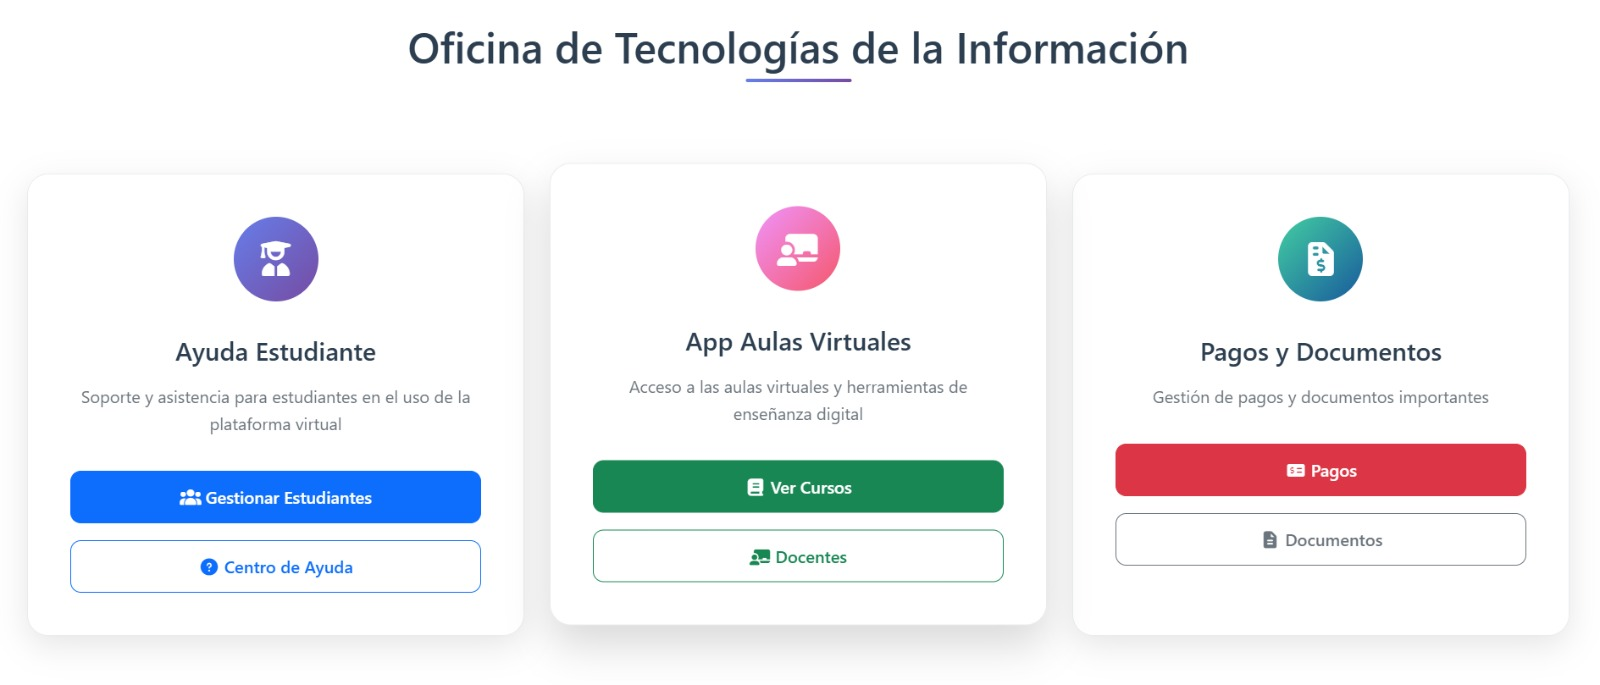
\includegraphics[width=0.8\textwidth]{images/login.jpeg}
    \caption{Vista de inicio de sesión del sistema}
\end{figure}

\begin{figure}[H]
    \centering
    
\includegraphics[width=0.8\textwidth]{images/welcome.jpeg}
    \caption{Pantalla principal de bienvenida al ingresar al sistema}
\end{figure}

\begin{figure}[H]
    \centering
    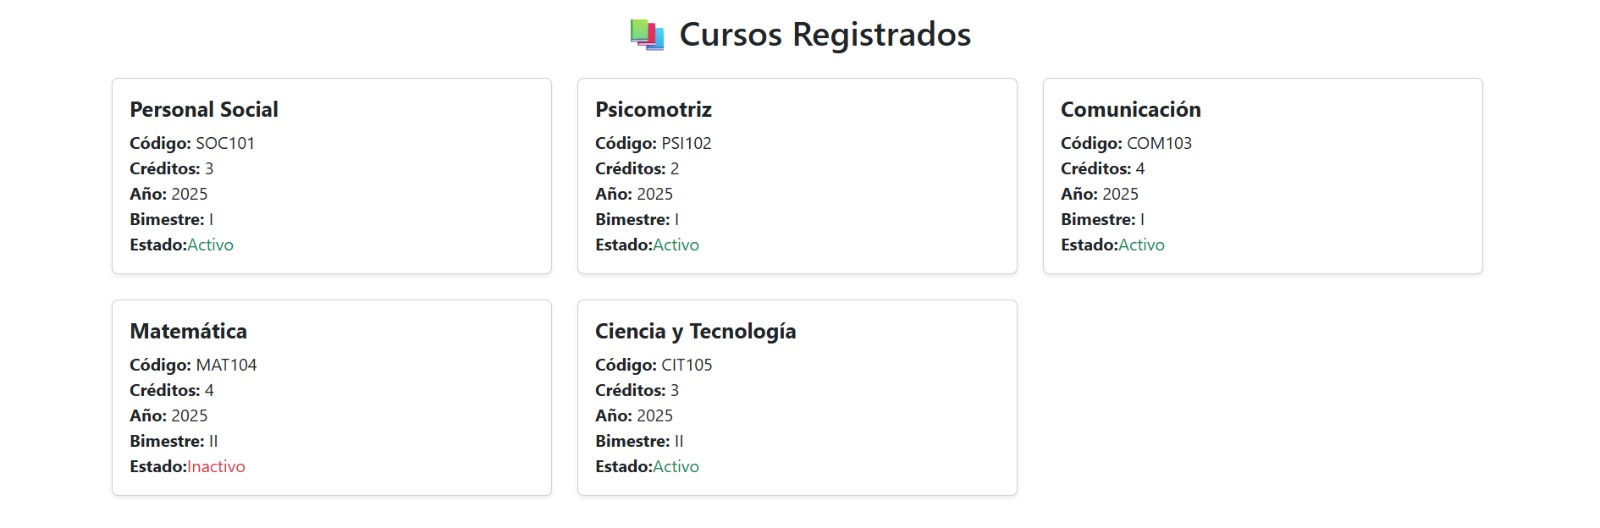
\includegraphics[width=0.8\textwidth]{images/cursos.jpeg}
    \caption{Sección de gestión de cursos para el usuario}
\end{figure}

\begin{figure}[H]
    \centering
    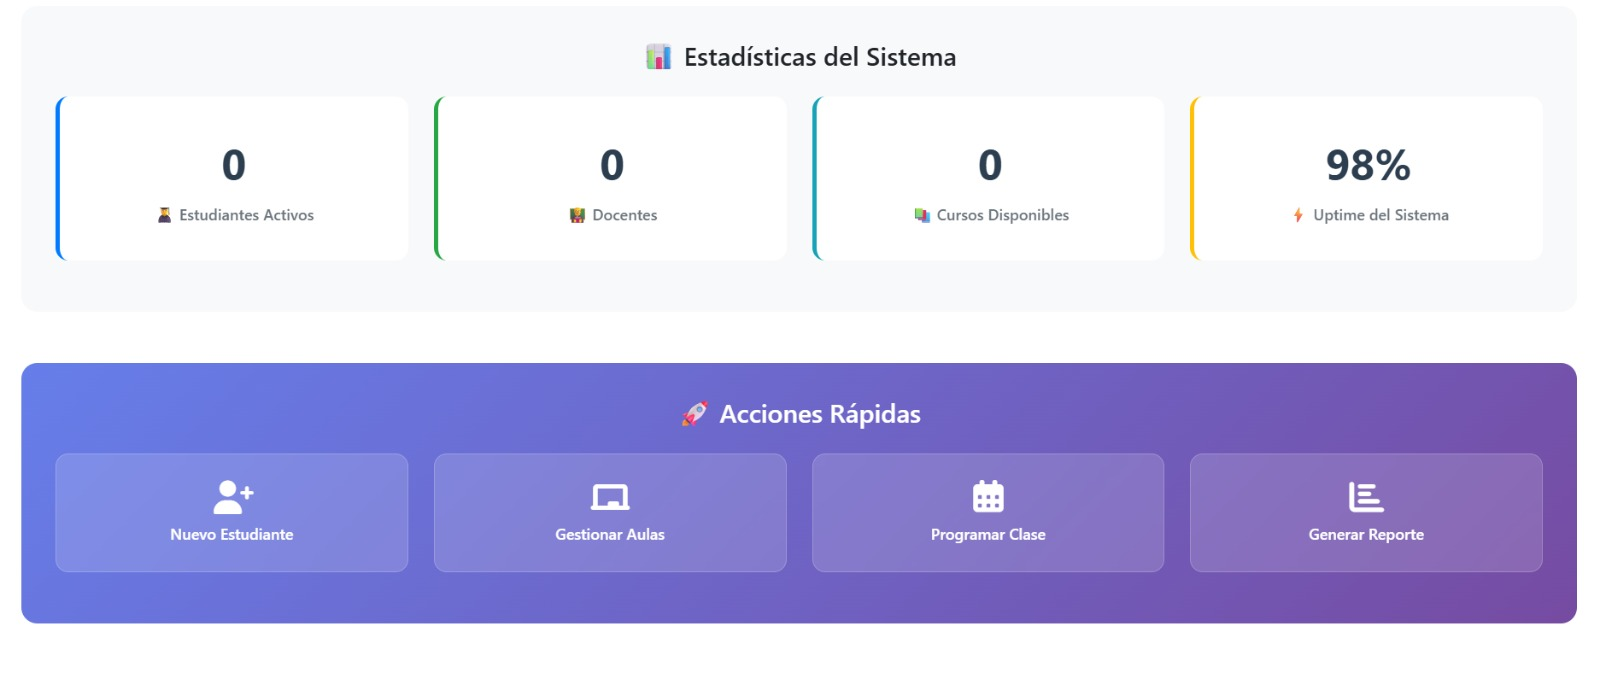
\includegraphics[width=0.8\textwidth]{images/admin.jpeg}
    \caption{Panel administrativo para usuarios con privilegios}
\end{figure}


    
\section{Despliegue del Proyecto}
    \subsection{Despliegue del Backend en Render}
        Para hacer accesible el backend desarrollado con Django, se utilizó la plataforma Render, la cual permite el despliegue continuo mediante la integración con GitHub. A continuación, se detallan los aspectos clave del despliegue:

        \begin{itemize}
            \item \textbf{Repositorio Git conectado:} Se enlazó el repositorio público del backend alojado en GitHub, disponible en la URL: \url{https://github.com/KarlaBedregal/CunaUnsa\_}.

            \item \textbf{Framework utilizado:} El proyecto fue desarrollado con Django y configurado para funcionar con una base de datos PostgreSQL remota, empleando variables de entorno para una mayor seguridad y portabilidad.

            \item \textbf{Archivo de entrada (entry point):} Render utiliza el archivo \texttt{manage.py} como punto de entrada para ejecutar las tareas administrativas del servidor.

            \item \textbf{Base de datos:} Se usó un servicio externo proporcionado por Supabase, el cual hospeda una instancia de PostgreSQL. La conexión se establece mediante variables de entorno definidas en la sección de configuración del servicio Render.

            \item \textbf{Variables de entorno configuradas en Render:}
            \begin{itemize}
                \item \texttt{DB\_NAME} = \texttt{postgres}
                \item \texttt{DB\_USER} = \texttt{postgres.zcsblgjwreggdewwdyxf}
                \item \texttt{DB\_PASSWORD} = \texttt{CunaUnsa-}
                \item \texttt{DB\_HOST} = \texttt{aws-0-us-east-2.pooler.supabase.com}
                \item \texttt{DB\_PORT} = \texttt{6543}
                \item \texttt{SECRET\_KEY} = \texttt{[clave secreta de Django]}
                \item \texttt{DEBUG} = \texttt{False}
                \item \texttt{ALLOWED\_HOSTS} = \texttt{["cuna-unsa-backend.onrender.com"]}
            \end{itemize}

            \item \textbf{Comandos de despliegue configurados:}
            \begin{itemize}
                \item \texttt{Build command:} \texttt{pip install -r requirements.txt}
                \item \texttt{Start command:} \texttt{gunicorn MyDjangoProject.wsgi}
            \end{itemize}

            \item \textbf{Estrategia de despliegue:} Se configuró el servicio como \texttt{Web Service}, con entorno \texttt{Python 3}, usando despliegue automático desde la rama principal (\texttt{main}) del repositorio.

            \item \textbf{URL pública del backend:} \url{https://cuna-unsa-backend.onrender.com} \\
            Esta URL permite a los clientes frontend y usuarios externos consumir la API REST del sistema desde cualquier ubicación.
        \end{itemize}

    \subsection{Despliegue del Frontend en Netlify}
        Para facilitar el acceso público a la interfaz del sistema, se utilizó la plataforma Netlify para el despliegue del frontend desarrollado en Vue 3.

        \begin{itemize}
            \item \textbf{Repositorio del Proyecto}: El código fuente del frontend se encuentra disponible en GitHub: \url{https://github.com/lau230595/CunaFrontend}{https://github.com/lau230595/CunaFrontend}
            
            \item \textbf{Configuración de Build}: Se configuró el archivo \texttt{netlify.toml} en la raíz del proyecto con las siguientes instrucciones:

            \begin{lstlisting}[language=bash, caption=Archivo netlify.toml]
[build]
command = "npm run build"
publish = "dist"

[[redirects]]
from = "/*"
to = "/index.html"
status = 200
            \end{lstlisting}
            
            \item \textbf{Comando de Build}: El comando de compilación para producción utilizado fue:

            \begin{lstlisting}[language=bash, numbers=none]
        $ npm run build
            \end{lstlisting}
            
            \item \textbf{Ruta de Publicación}: La carpeta generada tras el build es \texttt{dist}, la cual se especifica como carpeta a publicar en la configuración de Netlify.

            \item \textbf{Variables de Entorno}: Se requiere configurar una variable de entorno llamada \texttt{VUE\_APP\_API\_URL} para que el frontend se comunique con la API REST del backend desplegado.             
        \end{itemize}
    %%%%%
    \subsection{Conexión entre Frontend y Backend}

La comunicación entre el frontend (Vue 3) y el backend (Django + Django REST Framework) se realiza mediante peticiones HTTP a través de Axios, una librería JavaScript incluida como dependencia del proyecto.

\begin{itemize}
    \item \textbf{Archivo central de conexión:} En \texttt{src/services/api.js} se encuentra centralizada toda la lógica de consumo de la API. Allí se configura:
    \begin{itemize}
        \item La URL base de la API, leída desde una variable de entorno: \texttt{VUE\_APP\_API\_URL}.
        \item Interceptores de solicitud, que automáticamente añaden el token JWT a las cabeceras.
        \item Interceptores de respuesta, que manejan errores como expiración de sesión (401) y redireccionan al login.
        \item El envío del token CSRF en caso de ser necesario.
    \end{itemize}

    \item \textbf{Seguridad:} El backend entrega un \texttt{token JWT} tras el inicio de sesión. Este se almacena en el \texttt{localStorage} del navegador y se incluye en cada petición como cabecera \texttt{Authorization: Bearer <token>}. Esto asegura que el acceso a recursos protegidos sea autenticado.

    \item \textbf{Rutas consumidas:} Algunas rutas importantes del backend que el frontend utiliza son:
    \begin{itemize}
        \item \texttt{/api/auth/login/}, \texttt{/api/auth/logout/}, \texttt{/api/auth/profile/}
        \item \texttt{/api/students/}, \texttt{/api/teachers/}, \texttt{/api/courses/}, entre otras.
    \end{itemize}

    \item \textbf{Gestión desde componentes:} Los componentes Vue utilizan el archivo \texttt{api.js} para realizar las acciones necesarias. Por ejemplo, el componente \texttt{Login.vue} utiliza \texttt{api.login()} al enviar el formulario de inicio de sesión.

    \item \textbf{Configuración del entorno local:} En \texttt{vue.config.js} se configura un proxy local que redirige peticiones \texttt{/api} al dominio del backend en producción:
    \begin{lstlisting}[language=bash]
devServer: {
    proxy: {
        '/api': {
            target: 'https://cuna-unsa-production.up.railway.app',
            changeOrigin: true,
            secure: true,
        }
    }
}
    \end{lstlisting}
\end{itemize}

\textbf{Resumen:} La conexión entre ambas capas es robusta, segura y centralizada. Se asegura una integración fluida mediante uso de tokens, configuración modular y control automático de sesiones expiradas. Todo esto facilita la escalabilidad y el mantenimiento futuro del sistema.



    %%%%%
    \subsection{URLs Públicas del Sistema}
    A continuación se detallan los enlaces públicos relacionados al desarrollo, despliegue y documentación del sistema:
    \begin{itemize}
        \item \textbf{Repositorio del Frontend (Vue):} \url{https://github.com/lau230595/CunaFrontend}
        \item \textbf{Repositorio del Backend (Django):} \url{https://github.com/KarlaBedregal/CunaUnsa_}   
        \item \textbf{Sitio Web Desplegado (Netlify):} \url{https://cunaunsa.netlify.app/}
        \item \textbf{API REST Pública (Render):} \url{https://cunaunsa.onrender.com/api/}
        \item \textbf{Playlist de YouTube del Proyecto:} \url{https://www.youtube.com/playlist?list=PLxcXnsVAKkkOeRiS--BGBqqsqF3An7Tyf}
    \end{itemize}
  
\section{Trabajo en Equipo}
    \subsection{Distribución de Tareas}

\begin{itemize}
    \item \textbf{Bedregal Coaguila, Karla M.} —Desarrollo principal del backend en Django y API REST.
    \item \textbf{Llaique Chullunquia, Jack F.} — Desarrollo principal del frontend en Vue.
    \item \textbf{Ramos Ochochoque, Elkin E.} — Apoyo en documentación y backend.
    \item \textbf{Vilca Huarca, Laura L.} — Participación activa en backend, frontend y deploy de ambos.
\end{itemize}

    \subsection{Porcentaje de Participación}

\begin{center}
\begin{tabular}{|l|c|}
\hline
\textbf{Integrante} & \textbf{Porcentaje} \\
\hline
Bedregal Coaguila, Karla M. & 100\% \\
Llaique Chullunquia, Jack F. & 100\% \\
Ramos Ochochoque, Elkin E. & 100\% \\
Vilca Huarca, Laura L. & 100\% \\
\hline
\end{tabular}
\end{center}

    \subsection{Rubrica}
        \begin{table}[ht]
			\caption{Niveles de desempeño}
			\begin{center}
			\begin{tabular}{ccccc}
    			\hline
    			 & \multicolumn{4}{c}{Nivel}\\
    			\cline{1-5}
    			\textbf{Puntos} & Insatisfactorio 25\%& En Proceso 50\% & Satisfactorio 75\% & Sobresaliente 100\%\\
    			\textbf{2.0}&0.5&1.0&1.5&2.0\\
    			\textbf{4.0}&1.0&2.0&3.0&4.0\\
    		    \hline
			    \end{tabular}
		    \end{center}
	    \end{table}

       \renewcommand{\arraystretch}{1.3}
       \newpage
\begin{longtable}{|p{2.4cm}|p{2.5cm}|p{2.3cm}|p{2.3cm}|p{2.3cm}|c|c|}
\caption{Evaluación por Criterios} \\
\hline
\textbf{Criterio} &
\textbf{Excelente (3)} &
\textbf{Bueno (2)} &
\textbf{Regular (1.5)} &
\textbf{Deficiente (0.7)} &
\textbf{Auto} &
\textbf{Docente} \\
\hline
\endfirsthead

\multicolumn{7}{c}{{\bfseries \tablename\ \thetable{} -- continuación}} \\
\hline
\textbf{Criterio} &
\textbf{Excelente (3)} &
\textbf{Bueno (2)} &
\textbf{Regular (1.5)} &
\textbf{Deficiente (0.7)} &
\textbf{Auto} &
\textbf{Docente} \\
\hline
\endhead

\hline \multicolumn{7}{|r|}{{Continúa en la siguiente página}} \\ \hline
\endfoot

\hline
\endlastfoot

Producción de Videos &
Muy claro, estructurado. Alta calidad. &
Claro, buena calidad. Casi completo. &
Algo claro. Calidad media. &
Confuso o baja calidad. No comunica. &
 2 & \\
\hline

Backend en Producción &
Funciona sin errores. Seguridad sólida. &
Funciona con leves fallos. &
Parcialmente funcional. &
No funciona ni desplegado. &
 2 & \\
\hline

Frontend en Producción &
Interfaz funcional y atractiva. &
Usable con detalles menores. &
Interfaz básica, falta funcionalidad. &
Confuso o no funcional. &
 2 & \\
\hline

Backup de BD &
Completo, verificado y documentado. &
Completo pero sin prueba. &
Incompleto, manual. &
No hay backup. &
 2 & \\
\hline

GitHub Backend &
Commits claros. Buen uso de ramas. &
Organizado. Mensajes adecuados. &
Desordenado. Mensajes vagos. &
Caótico. Todo en main. &
 2 & \\
\hline

GitHub Frontend &
Estructura clara y ramas activas. &
Constante, sin mucho detalle. &
Básico y directo a main. &
Sin estructura ni control. &
 2 & \\
\hline

Informe Final &
Completo, análisis crítico. &
Buen análisis, pocos errores. &
Cumple, con algunos errores. &
Incompleto o con errores graves. &
 2 & \\
\hline

\textbf{Total (/21)} & & & & & 14 & \\
\hline
\end{longtable}


\section{Conclusiones}

\begin{thebibliography}{00}

\bibitem{vue-docs}
Vue.js, “Vue.js Guide,” [Online]. Available: \url{https://vuejs.org/guide/introduction.html}. [Accessed: 27-Jul-2025].

\bibitem{vuex-docs}
Vuex, “State Management for Vue.js,” [Online]. Available: \url{https://vuex.vuejs.org/}. [Accessed: 27-Jul-2025].

\bibitem{axios-docs}
Axios, “Axios HTTP Client,” [Online]. Available: \url{https://axios-http.com/docs/intro}. [Accessed: 27-Jul-2025].

\bibitem{vue-router}
Vue Router, “Vue Router Official Docs,” [Online]. Available: \url{https://router.vuejs.org/}. [Accessed: 27-Jul-2025].

\bibitem{drf-docs}
T. Christie, “Django REST framework,” [Online]. Available: \url{https://www.django-rest-framework.org/}. [Accessed: 27-Jul-2025].

\bibitem{django-docs}
Django Software Foundation, “Django Documentation,” [Online]. Available: \url{https://docs.djangoproject.com/en/stable/}. [Accessed: 27-Jul-2025].

\bibitem{netlify-docs}
Netlify, “Netlify Documentation,” [Online]. Available: \url{https://docs.netlify.com/}. [Accessed: 27-Jul-2025].

\bibitem{render-docs}
Render, “Render Docs,” [Online]. Available: \url{https://docs.render.com/}. [Accessed: 27-Jul-2025].
\bibitem{bootstrap-docs}
Bootstrap, “Bootstrap 5 Documentation,” [Online]. Available: \url{https://getbootstrap.com/docs/5.3/getting-started/introduction/}. [Accessed: 27-Jul-2025].

\bibitem{jwt-docs}
Auth0, “Introduction to JSON Web Tokens,” [Online]. Available: \url{https://auth0.com/docs/secure/tokens/json-web-tokens}. [Accessed: 27-Jul-2025].

\bibitem{eslint-docs}
ESLint, “ESLint Documentation,” [Online]. Available: \url{https://eslint.org/docs/latest/}. [Accessed: 27-Jul-2025].

\bibitem{vue-cli}
Vue.js Team, “Vue CLI - Standard Tooling for Vue.js Development,” [Online]. Available: \url{https://cli.vuejs.org/}. [Accessed: 27-Jul-2025].

\end{thebibliography}



%%%%%%%%%%%%%%%%%%%%%%%%%% FIN CUERPO DEL INFORME %%%%%%%%%%%%%%%%%%%%%%%%%%
    \end{document}
%SUBIR IMAGENES
begin{figure}[H]
    \centering
    \includegraphics[width=0.7\textwidth]{"nombre del archivo"}
    \caption{"Nombre para la imagen"}
\end{figure}

%SUBIR CODIGO
\begin{lstlisting}[language=Python, caption={Modificar settings.py}]
(aca va el codigo a mostrar equide)
\end{lstlisting}